\documentclass[12pt,mscthesis]{usiinfthesis}

\usepackage{lipsum}
\usepackage{graphicx}
\usepackage{float}
\usepackage{cleveref}
\graphicspath{ {figures/} }

\usepackage{listings}
\usepackage[autostyle]{csquotes} 

\lstdefinelanguage{algebra}
{morekeywords={import,sort,constructors,observers,transformers,axioms,if,
else,end},
sensitive=false,
morecomment=[l]{//s},
}



\title{Assessing Documents by Comprehension Effort } %compulsory
%\specialization{Dependable Distributed Systems}%optional
%\subtitle{Subtitle: Reinventing the World} %optional 
\author{Talal El Afchal} %compulsory
\begin{committee}
\advisor{Prof.}{Michele}{Lanza} %compulsory
\coadvisor{Prof.}{Gabriele}{Bavota}{} %optional
\coadvisor{Dr.}{Luca}{Ponzanelli}{}

\end{committee}
\Day{1} %compulsory
\Month{September} %compulsory
\Year{2017} %compulsory, put only the year
\place{Lugano} %compulsory

\dedication{To my beloved} %optional
\openepigraph{Your living is determined not so much by what life brings to you as by the attitude you bring to life; not so much by what happens to you as by the way your mind looks at what happens}{Gubran Khalil Gubran} %optional

%\makeindex %optional, also comment out \theindex at the end

\begin{document}

\maketitle %generates the titlepage, this is FIXED

\frontmatter %generates the frontmatter, this is FIXED

\begin{abstract}
Recommender systems for software developers have become increasingly popular in recent years. These systems combine several methodologies to provide suggestions that meet the developer's needs. The recommender systems collect data from online resources as blogs, forums, Q\&A websites, and suggest documents or piece of code that are most likely helpful to the developers. However, these systems are not taking into consideration an important aspect as the comprehension effort, which may vary depending on the document familiarity and readability. Usually developers are more interested in documents which they are familiar with. By calculating the comprehension effort, the recommender system can re-rank the documents and suggest the most comprehensive and appropriate ones to the developer. In this work, we present our approach to calculating the comprehension effort, by creating a language model able to capture a document familiarity, that we combine with the document readability. 
\end{abstract}

\begin{acknowledgements}
\end{acknowledgements}

\tableofcontents 
\listoffigures %optional
\listoftables %optional

\mainmatter

\chapter{Introduction}

	\section{Context}
	The complexity of software systems is increasing, and to make them less complex, new technologies are introduced constantly. Software developers often have to work with new technologies which they are not familiar with, and as increasingly more comes out, the amount of information that they need to know will increase. Android\footnote{url{https://www.android.com}}, for example, was introduced 10 years ago in 2007. Nowadays, there are more than three million applications available on the Google store. \\
	When Android started to become popular, developers had to learn this technology and to stay updated with each new version release. 
	They had to figure out how activities work in Android, and how to use several APIs to implement different tasks assigned to them. Where do they start from? Is there some tutorial on the web where they can learn how to use a specific API? Where can they find a piece of code that can be reused in their application? \\
	Google is the most popular search engine, where an \emph{Android tutorial} query search, we will return 22 million documents\footnote{\url{https://www.google.ch/search?site=&source=hp&q=android+tutorial&oq=android+tutorial}}, even if we search for a specific field, as an Android Bluetooth tutorial\footnote{\url{https://www.google.ch/search?client=safari&rls=en&biw=1440&bih=839&q=android+bluetooth+example}}, we get 6 million documents which still a huge number.\\
	Stack Overflow is one of the most popular Q\&A websites for developers, where a million of questions are tagged as Android\footnote{\url{https://stackoverflow.com/questions/tagged/android}}. \\
	Github is one of the most popular version control system, where developers can store their projects, and it hosts more than 500 thousand Android repositories\footnote{\url{https://github.com/search?utf8=✓&q=android&type=}}, with millions of lines of code. Those numbers are gigantic, and it is obvious that finding the most suitable document is not obvious, since given the big number of available documents it is not feasible for the developer to check all of them and choose the right one.\\
	To overcome this problem, recommender systems for software engineering were introduced as an important support for programmers. They provide the most valuable documents in a given context.\\

	The proposed definition by the organizers of the ACM International Conference on Recommender Systems:\footnote{\url{https://recsys.acm.org/recsys09}} \\

	  \blockquote{\textit{``Recommendation systems are software applications that aim to support users in their decision-making while interacting with large information spaces. They recommend items of interest to users based on preferences they have expressed, either explicitly or implicitly. The ever-expanding volume and increasing complexity of information [...] has therefore made such systems essential tools for users in a variety of information seeking [...] activities. Recommendation systems help overcome the information overload problem by exposing users to the most interesting items, and by offering novelty, surprise, and relevance.''}}
	Now that we defined what is a recommender system, we can mention \citet{RecommendationSystemsforSoftwareEngineering} definition of the recommender systems for software engineering (RSSE):\\

	\textbf{An RSSE is a software application that provides information items estimated to be valuable for a software engineering task in a given context.}\\

	The RSSE definition highlights the importance of the \textbf{context} and the \textbf{valuable information}, therefore RSSEs are an important support for programmers to find the information they should know, and the RSSEs have to consider and evaluate alternative decisions. We believe that the effort to comprehend a document must be a part of the document evaluation.\\


	Searching for documentation and tutorials is a crucial step in learning a new technology. The developers can find a bunch of online resources as blogs, forums, Q\&A websites, but the real challenge is to find the most suitable one for their needs.



	\citet{Singer-1997} reported in 1997 that the most frequent developer activity was code search, and \citet{Sadowski:2015} did a case study on how developers at Google search for code. They figured out that programmers are generally seeking answers to questions about how to use an API, what code does, why something is failing, or where the code is located. The interesting point in this study was the fact that most searches focus on code that is familiar, or somewhat familiar to the developers.\\
	Therefore, we believe that recommender systems for software developers have to take into consideration the familiarity of a document when they suggest it to the developer. 


	Understanding a document is a cognitive process, and it depends on the human brain intelligence, but we all agree that if we are familiar with a subject, we will comprehend it with less effort. A computer engineer comprehends a document that explains how to implement a sorting algorithm, with much less effort compared to a document that explains a constitutional law, and the reason is not that the algorithm is not complex, but because a computer engineer is more familiar with sorting algorithms.\\
	
	In this thesis, we try to evaluate less trivial situations, for example:\\
	Given two documents that have approximately the same subject, how can we decide which one is easier to comprehend?\\
	In order to answer this question we need to introduce two concepts:
	\begin{itemize}
	\item \textbf{familiarity}: how much are a developer familiar with the document content?
	\item \textbf{readability}: how difficult is it to read a given document?
	\end{itemize}
	The comprehension effort can be derived from the document familiarity and readability.\\

	For example, if we want to use a tool that gives us a score to indicate which document requires less effort to be comprehended, where a higher score indicates a high effort. And we have two documents where, in the first one we have a sorting algorithm implemented in Java, and in the second one a sorting algorithm implemented in Fortran, and the developer is more familiar with Java.\\
	We expect that the first document must have a lower score since logically it requires less effort to be comprehended by developers who are more familiar with Java.
	What if both documents have a sorting algorithm implemented in the same programing language? Which one will have a lower score? \\
	In this case, the document readability has a big impact on the comprehension effort:\\
	The developer would likely prefer to read the document with the best readability.\\
	
	\section{Objective and Results}
	Our main goal in this thesis is to assess documents by their comprehension effort, which can be leveraged by RSSE to improve their suggestions.\\
	To calculate the comprehension effort we need to find a way to calculate the familiarity, and we need to evaluate our approach to understand if it effectively works.\\

	 As a first step, we select a big set of Android documents, which represents the hypothetical developer knowledge, where a document can be a mix of code and natural language. Then we create a \emph{ Language Model} \cite{Hindle:2012:NS:2337223.2337322} and we train it with these documents (training documents). In this way, we are able to simulate a programmer who is familiar with Android. Once we trained the language model, we evaluate the familiarity of a given set of documents (testing documents) that contains Android documents and other documents that are not related to Android.\\ 
	 The language model was able to evaluate the Android testing documents as thousand times more familiar than the rest of the testing documents.
	 In this experiment, the language model approach satisfied our expectation in capturing the document familiarity.\\

	 On the top of this experiment, we did a case study to evaluate our approach in assessing documents by the comprehension effort. In this study we ask programmers to read a set of tutorials, and then we give them a set of documents, where some documents are related to the tutorials and some are not.
	 \newpage
	 The developers are just asked to score the documents by the comprehension effort on a scale from 1 to 5 (1$-$low effort 5$-$high effort)
	 \dots 
	

	\section{Structure of the Thesis}
	This thesis consists of seven chapters: 
	\begin{enumerate}
	
		\item \textbf{Introduction}: In this chapter we introduce the thesis work.
		\item \textbf{State of the Art}: This chapter describes the existing related work as code search engines, and recommender systems.
		\item \textbf{Approach}: This chapter describes our approach to calculate the comprehension effort.
		\item \textbf{Study design}: This chapter discusses the research question, the data extraction process, the analysis method, and the replication package.
		\item \textbf{Result}: This chapter shows the results and their implication.
		\item \textbf{Threat to Validity}: This chapter describes our assumptions, and the possible threats that could affect the results validity.
		\item \textbf{Conclusion}: This chapter is a summarization of our work, where we present some ideas for a possible future work.
	\end{enumerate}
\chapter{State of the Art}
	In this chapter, we talk about the existing related work to the comprehension effort, and we talk about code search engines and recommender systems.\\ 
\section{Comprehension}
	\citet{Kushwaha:2006:ICI:1163514.1163533} introduced a new equation :\\
	\begin{center}
	 \textbf{Difficulty in understanding the software}\\
	 \approx\\
	  \textbf{Difficulty in understanding the information}
	  \end{center}

	They claim that the required effort to understand a software depends on the difficulty in understanding the information, where the information is related to the number of operators and identifiers. They calculate the number of operators and identifiers per line of code and they multiply it by an associated weight of the identifier name ( 1 if the identifier name belongs to the problem domain, and 4 is the identifier name is selected arbitrarily). \\
	They performed an experiment on 60 students, where 5 sample programs were given. One set of programs had meaningful identifier names related to the problem domain and the other used arbitrarily selected identifier name. They measured the required time to comprehend the program.\\ 
	The result showed that programs with arbitrarily selected identifier names required about 4 times the time to comprehend the programs compared to programs with meaningful identifier names.\\



	\newpage
	\citet{Scalabrino}tried to introduce a metric able to assess the understandability of a given snippet code. In their work they consider three types of metrics:
	\begin{enumerate}
		\item \textbf{Code-related metrics} are metrics related to the code, as cyclomatic complexity, LOC, the number of identifiers, line length and many other metrics.
		\item \textbf{Documentation-related metrics} capture the quality of the internal documentation of a snippet (comments readability, and identifiers consistency). 
		\item \textbf{Developer-related metrics} measure the programming experience of the developer in years, in any programming language.
	\end{enumerate}
	They analyze whether code-related, documentation-related, and developer- related metrics can be used to assess the understandability level of a snippet  code.
	46 developers participated in this study. They were asked to carefully read and to fully understand eight code snippets. Participants could, in any moment select the option \textit{I understood the snippet} or \textit{I cannot understand the snippet}, and the time was monitored.
	Once the participant chooses \textit{I understood the snippet} option they ask question about the snippet code to verify the actual level of understanding.\\ 
	\textit{``After an extensive statistical analysis, none of the considered metrics exhibit a significant correlation with the understandability of code snippets''.}\\
	They assumed that the code complexity has a big influence on the programmers' ability to understand the code, but they couldn't demonstrate it with a strong empirical evidence.\\
	They also mentioned that the code readability can have a direct impact on the understandability of the code.\\ As mentioned in the previous chapter, in this thesis the code readability is a part of our comprehension effort calculation.\\

	\citet{Buse2010} introduced a code readability metric, and they investigate its relation to software quality. A part of their work was to run an experiment which compares readability of the code to the cyclomatic complexity, and they were able to validate that the code readability is significantly independent of the traditional code complexity.\\
	In this experiment, 120 developers were asked to individually score a sequence of 100 code snippets, based on their personal estimation of readability. From the result, they determined which code features are predictive of readability, and they construct a readability model. They also tested the model performance on ten different classifiers, and on average the model classified correctly between 75\% and 80\% of the snippets.\\
	They found that factors like \textit{average line length} and, \textit{average number of identifiers per line} are very important to readability.\\
	In this thesis we use \citet{Buse2010} approach to calculating code readability.

	\section{Semantics Code Search}

	\citet{Reiss:2009:SCS:1555001.1555040} presented a tool that generates a specific functions or classes from the open source repositories, where these classes meet user's specifications. This tool uses the user's input, as keywords and other constraints, and suggests codes that meet the user's needs.\\
	The tool takes a set of candidate solutions, and it transforms it into a more appropriate set. Both static and dynamic specifications can be used.\\
	This tool main goal is to satisfy the user's constraint, but it doesn't take into consideration the user's experience or the comprehension effort.\\
	

	\citet{Thummalapenta:2007:PPA:1321631.1321663} presented a tool similar to \citet{Reiss:2009:SCS:1555001.1555040}, where they collect code from public sources and they suggest it to the programmer based on their input query.\\ In the query, the programmers have to specify the \textit{source object type} and the \textit{destination object type}.\\ This tool is too restrictive and doesn't take into consideration any readability or complexity metrics.\\

	\citet{McMillan:2011:FRF:1985793.1986032} created an application search system called \textit{Exemplar}, which reduce the mismatch between the high-level intent reflected in the descriptions of software and low-level implementation details.\\ Exemplar differs from the traditional search engine that matches the keywords, by matching keywords with the descriptions of the various API calls in help documents.\\
	Exemplar has three components of Ranking: 
	\begin{enumerate}
		\item \textbf{WOS} a component that computes a score based on word occurrences in project descriptions
		\item \textbf{RAS} a component that computes a score based on the relevant API calls
		\item \textbf{DCS} a score based on data-flow connections between calls
	\end{enumerate}
	In this paper \citet{McMillan:2011:FRF:1985793.1986032}  said : \\
	\textit{``the results suggest that the performance of software search engines can be improved if those engines consider the API calls that the software uses.''}

	\section{Code Search Engines}
	\citet{Bajracharya2012} conducted an exploratory analysis of the usage log of Koders, the first commercially available Internet-Scale code search engine, and their goal is to answer the following three questions:\\
	\begin{enumerate}
	\item \textbf{Usage}: What kind of usage behavior can we see in Koders?
	\item \textbf{Search Topics}: What are the users searching for?
	\item \textbf{Query Forms}: How are users expressing their information need in their queries?
	\end{enumerate}
	They start analyzing the usage logs, and they get the following results: 
	\begin{itemize}
	\item Most of the users did not use Koders again after using it for a day
	\item Sessions are short (a series of activities by a single user within a small duration of time constitutes a session )
	\item More than half of the sessions had no downloads
	\item There are few sessions with no search activities
	\item Queries are very short
	\item Terms in queries are quite diverse
	\item Code queries are the mostl used types of queries
	\item Code queries lead to the most of the downloads
	\end{itemize}
	they conclude the analysis by mentioning that usage behavior is similar between Koders and search on the Web, and the majority of the users don't refine their existing queries.\\
	\newpage
	
	\section{Libra}
	\citet{Ponz2017a} created LIBRA, a holistic recommender system that supports developers in their information search in the web browser. The developers are tracked during their activities in the IDE and in the web browser, which allows Libra to collect information as web search results, perused pages, and code written and modified by the developer. LIBRA uses this information to model a knowledge context of the developer and, constructs a holistic meta-information model of their contents.\\
	
	LIBRA is based on three important metrics :
	
	\begin{itemize}
	\item \textbf{Context Complementarity} measures the information intake provided by a resource in the current context of the developer. A low context complementarity indicates that the resource information is already a part of the context.In other words, the resource and the context are too similar, and the amount of new information that the developer can retrieve is low.
	
	\item \textbf{Result Prominence} identifies prominent results among the search engine result set. When a query matches a result, it doesn't tell us so much about the result relevance. If a result overlaps with many other results, it would be more prominent, since probably it provides diversified information in its contents.
	
	\item \textbf{Information Quantity} sums up the number of ``elements'' identified by LIBRA's meta-information system. This metric is important to distinguish which resource has more information giving two resources with a similar number of characters. If the first resource has only text and the second one has text and code, obviously the second resource contains a higher information quantity.
	\end{itemize}

	16 3rd year CS Bachelor students were asked to evaluate LIBRA in terms of \textit{its ability in correctly assessing for each query search result its prominence and complementarity with respect to the context, and usefulness to developers during a development or maintenance task.}\\
	The study results indicated that both prominence and complementarity indicators reflect developers’ perception of such measures, and are considered as useful indicators. Moreover, with LIBRA the students  achieved a significantly better task completeness.\\

	The work that has been done in this thesis can be integrated with LIBRA, where the comprehension effort metric can be added to the other three metrics used by LIBRA.


\chapter{Approach}
	The volume of online resources is increasing, we can find millions of documents related to one search query. However, how can we suggest the most suitable one to developers? Several elements determine which documents contain valuable information, and one of these elements is the comprehension effort.\\
 The most frequent developer activity is code search \cite{Singer-1997}, and most searches focus on code that is familiar to the developer\cite{Sadowski:2015}. Certainly, developers prefer to search for documents they are familiar with since they require less effort to be comprehended. We believe that the comprehension effort is strictly related to the document familiarity and readability.\\
 So far many studies were done on the text readability (Flesch$-$Kincaid, Dale$-$Chall), and code readability \cite{Buse:2010:LMC:1850489.1850615}, but in this thesis, we introduce for the first time a new approach to calculate a document familiarity.\\

	
	
	\begin{figure}[htbp]
	\centering
	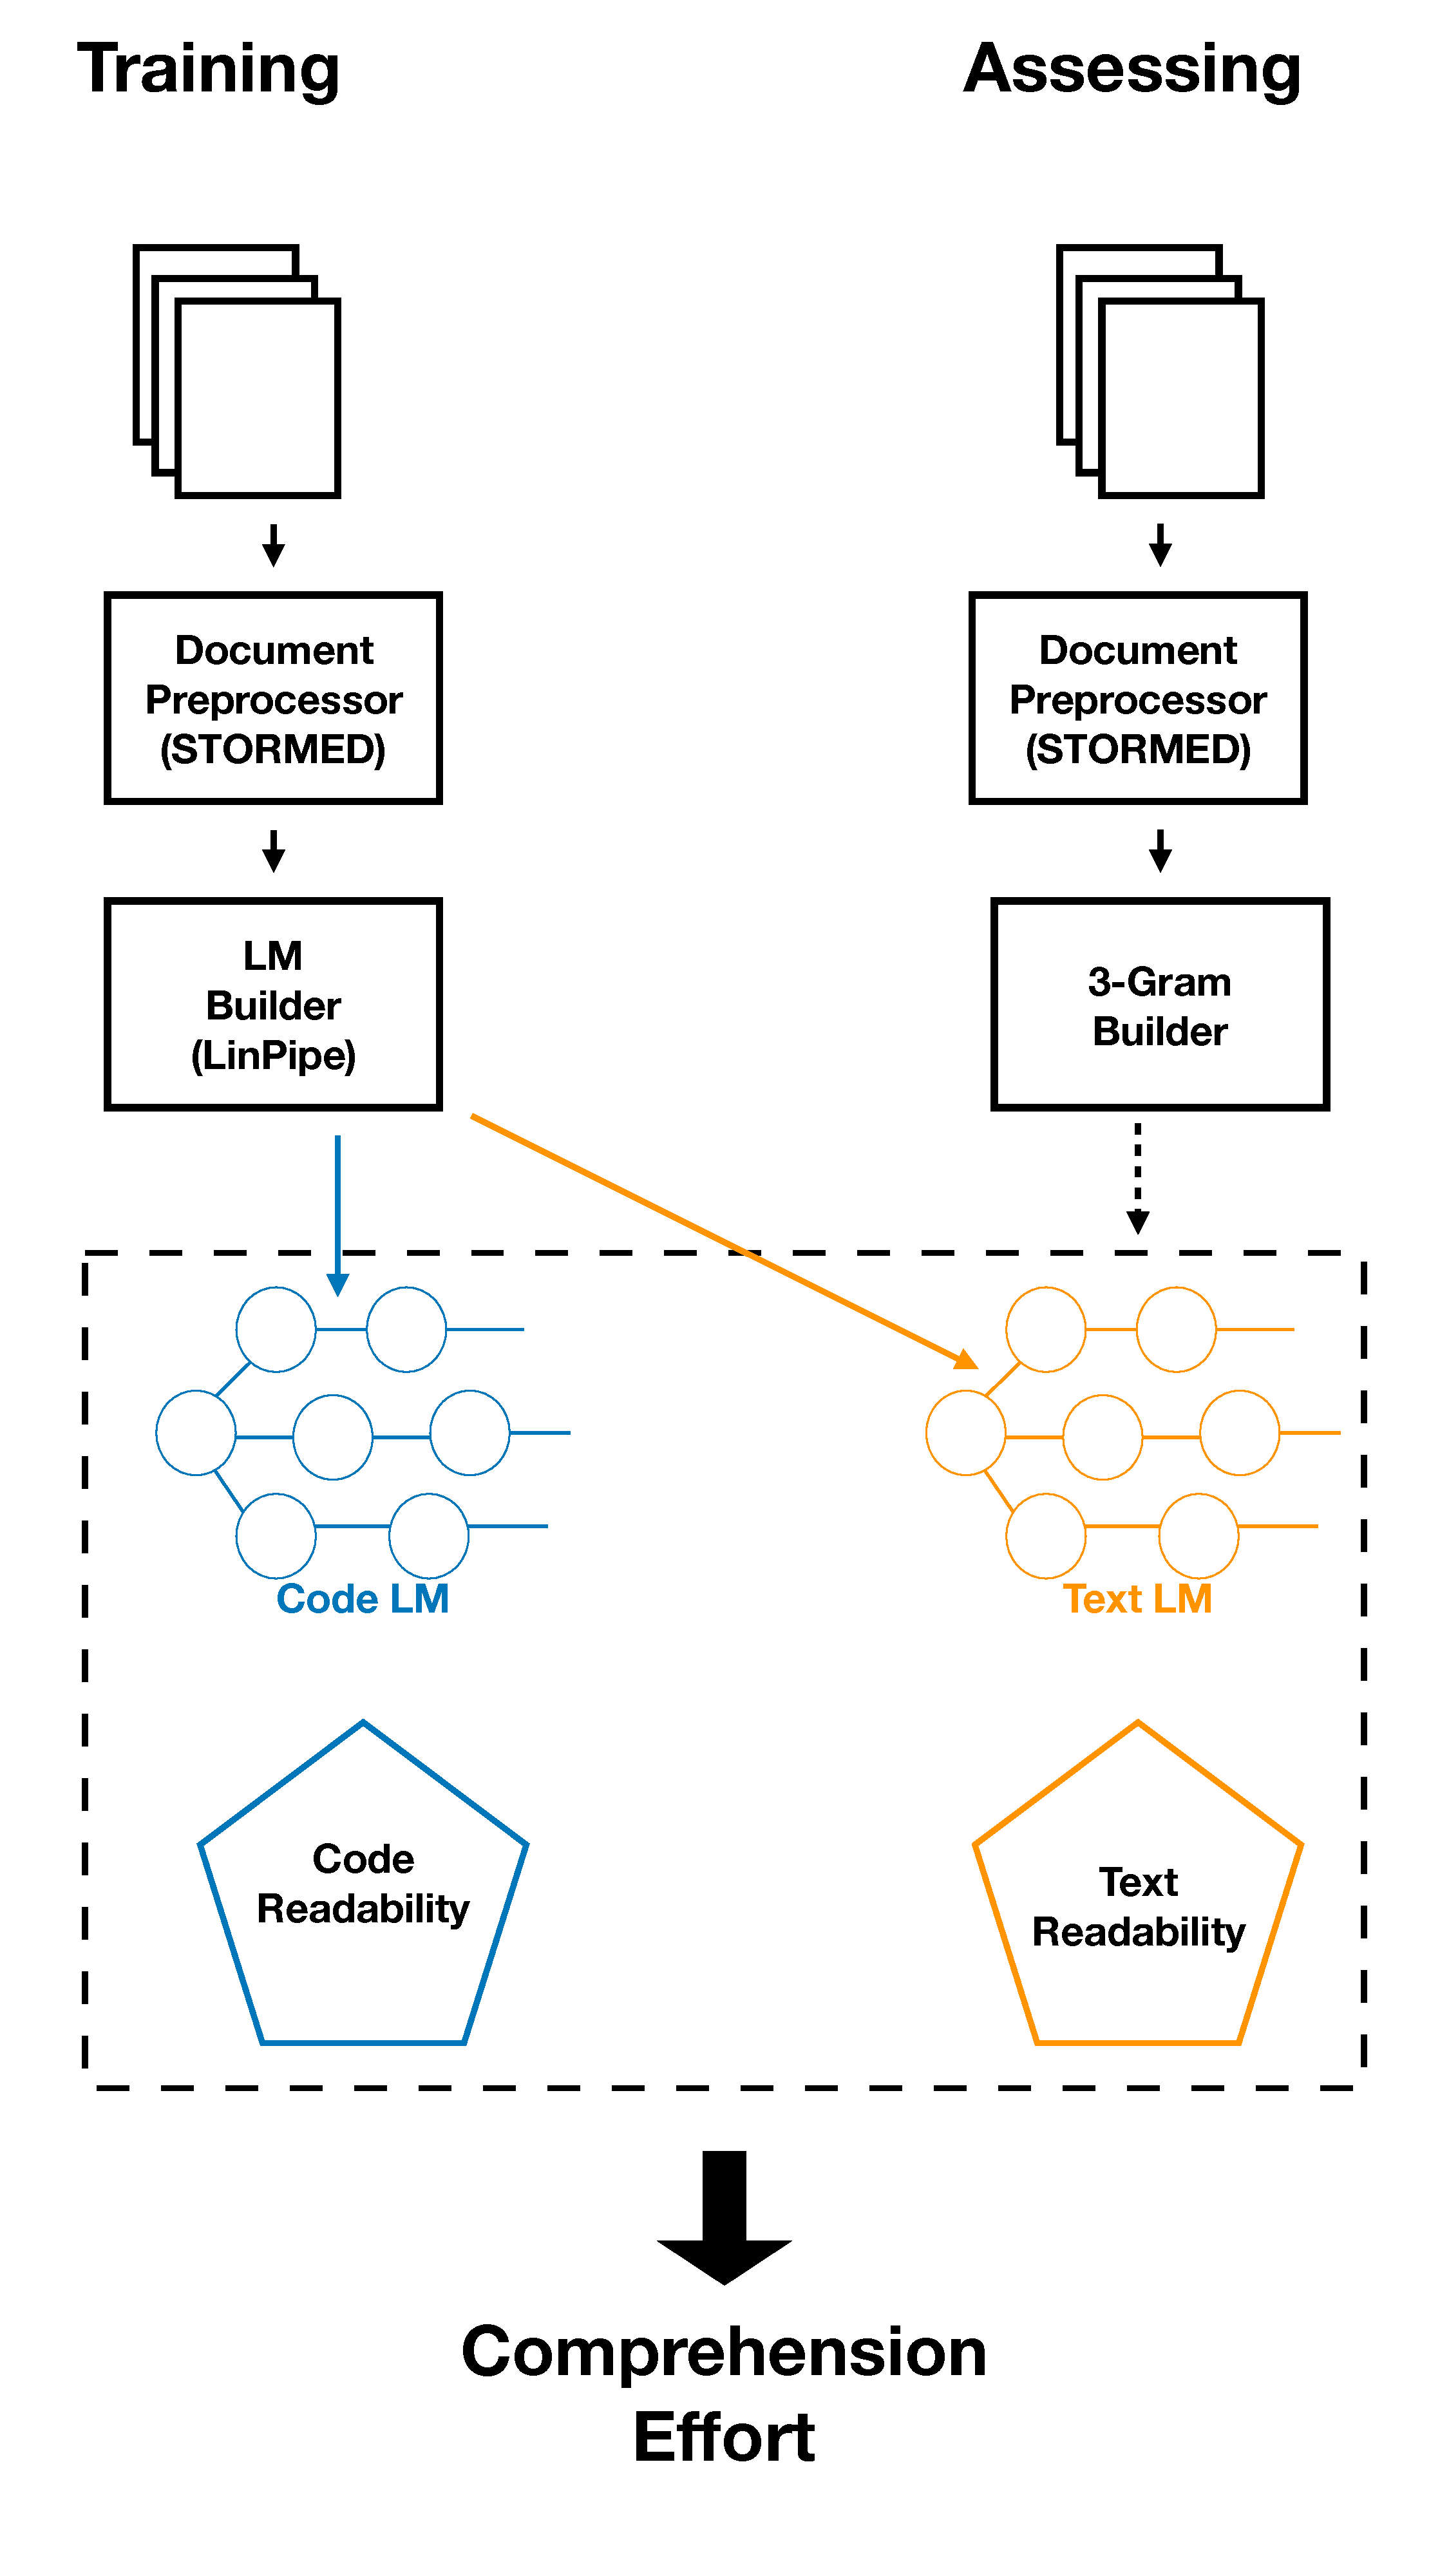
\includegraphics[width=12cm, height=\textheight]{overview}
	\caption{Overall architecture of our approach}
	\label{overview}
	\end{figure}
	\newpage
\section{Overview}

	\cref{overview} shows the overall architecture of our approach. As we can see, we have two \emph{language models}, one for code and one for text (natural language), and the whole process can be seen as two phases that work in parallel: 
	\begin{itemize}
		\item \textbf{Assessing phase}  Each document contains natural language or code or both of them, therefore, we calculate the readability and the familiarity separately as shown in \cref{fig1}. 
		In order to extract code and natural language from a document, we use Stormed Island Parser\footnote{\url{https://stormed.inf.usi.ch}} \cite{Ponz2015a}.\\
		On the other hand, we use a language model to calculate the familiarity of a document, Flesch$-$Kincaid to calculate the text readability, RayKernel \cite{Buse:2010:LMC:1850489.1850615} to calculate the code readability.
		\item \textbf{Training phase} where each document is broken down in two segments: code and text. The \emph{code language model} will be trained with the code segment, and the \emph{text language model} will be trained with the text segment.
	\end{itemize}

	\begin{figure}[htbp]
	\centering
	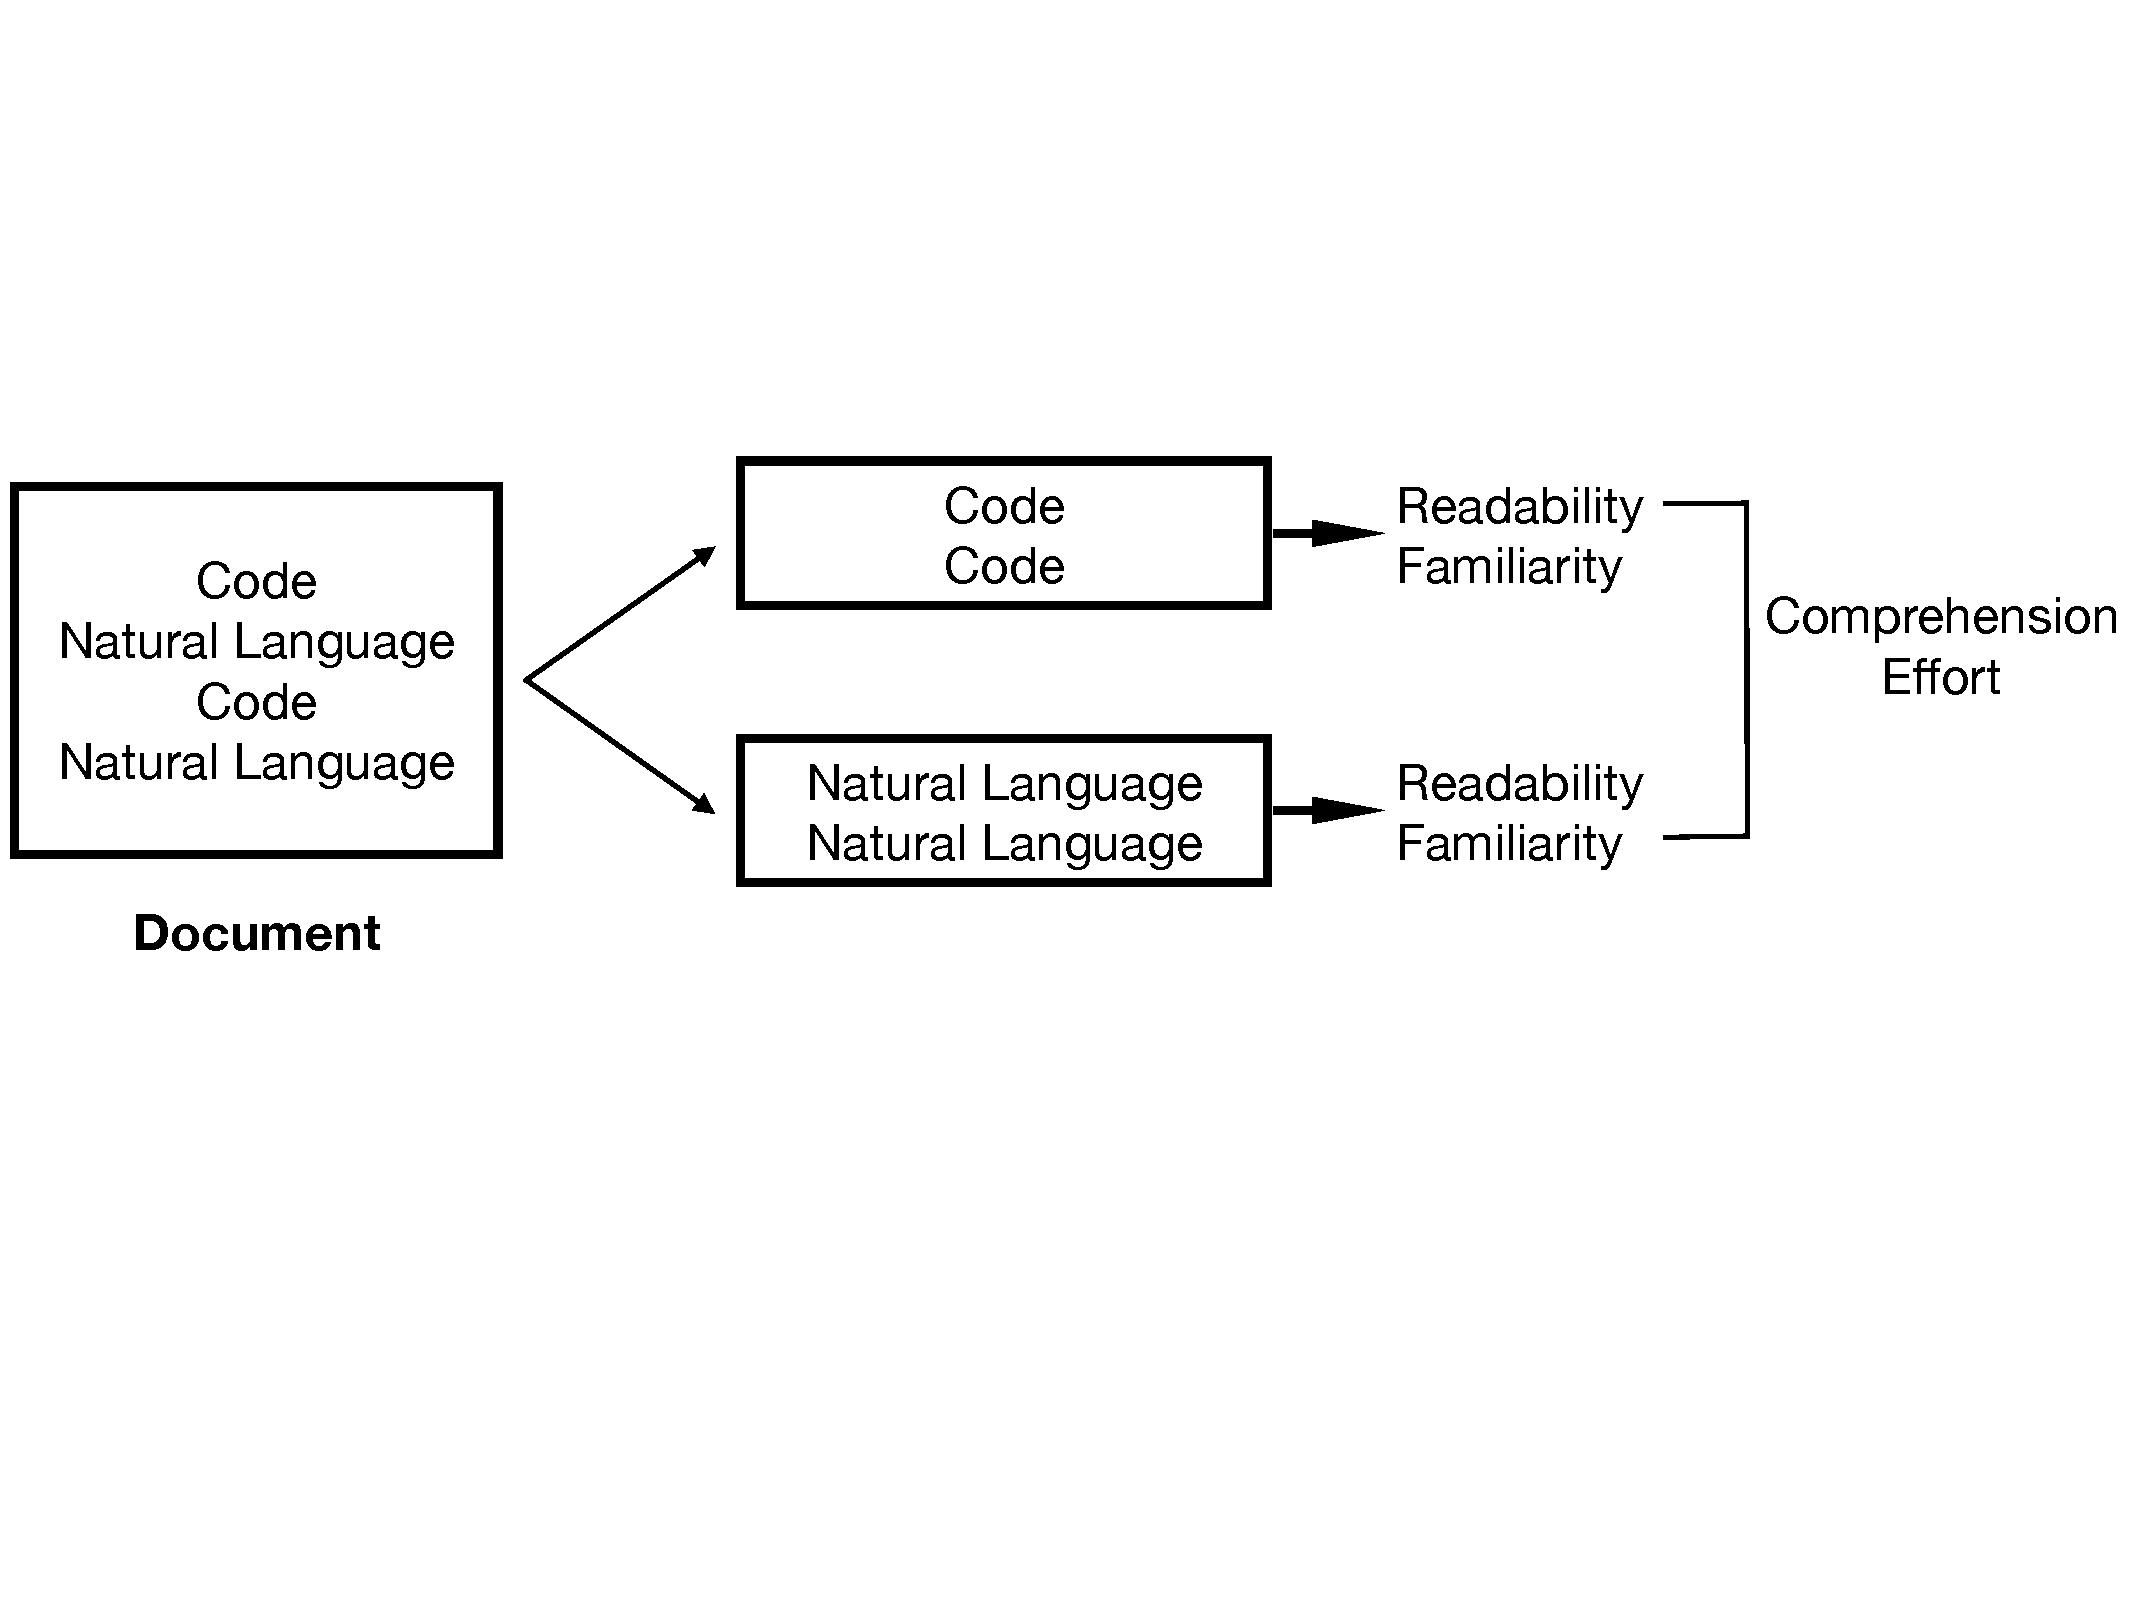
\includegraphics[width=\textwidth]{fig1}
	\caption{Document accessing}
	\label{fig1}
	\end{figure}

	In the next sections we explain the training and assessing phase, and we give more details about the component that are used in the whole process.

\newpage
	\section{Stormed Island Parser}
	
	 Stormed is a dataset for Stack Overflow that models the posts by building a heterogeneous abstract syntax tree H-AST for each discussion in the data dump \cite{Ponz2015a}.  The H-AST nodes model the contents of a Stack Overflow discussions according to the kind of structured fragment it represents. As shown in \cref{stackOverflow} each Stack Overflow document is represented with HTML tag, Stormed extracts two types of information units:
	 	 \begin{itemize}
		\item \textbf{Text Unit}: textual part of a discussion. Text units are all fragments that are not tagged as <code>	
		\item \textbf{Structured Fragment Unit}: code part of a discussion. Structured Fragment Unit are every contents tagged as <code> 
	 \end{itemize}

	 In \cref{stormed} we can see that Stormed gives us more detailed information about the \textit{Structured Fragment Unit}.\\
	 Each \textit{Structured Fragment Unit} can be one of the following possible structured fragments:
	 \begin{itemize}
	 \item \textbf{JavaASTNode}: Java code including incomplete fragments.
	 \item \textbf{StackTracesASTNode}: stack traces including incomplete stack trace lines.
	 \item \textbf{XMLASTNode}: XML/HTML documents, tags and elements.
	 \item \textbf{JSONASTNode}: JSON fragments.
	 \end{itemize}


	\begin{figure}[htbp]
	 \centering
	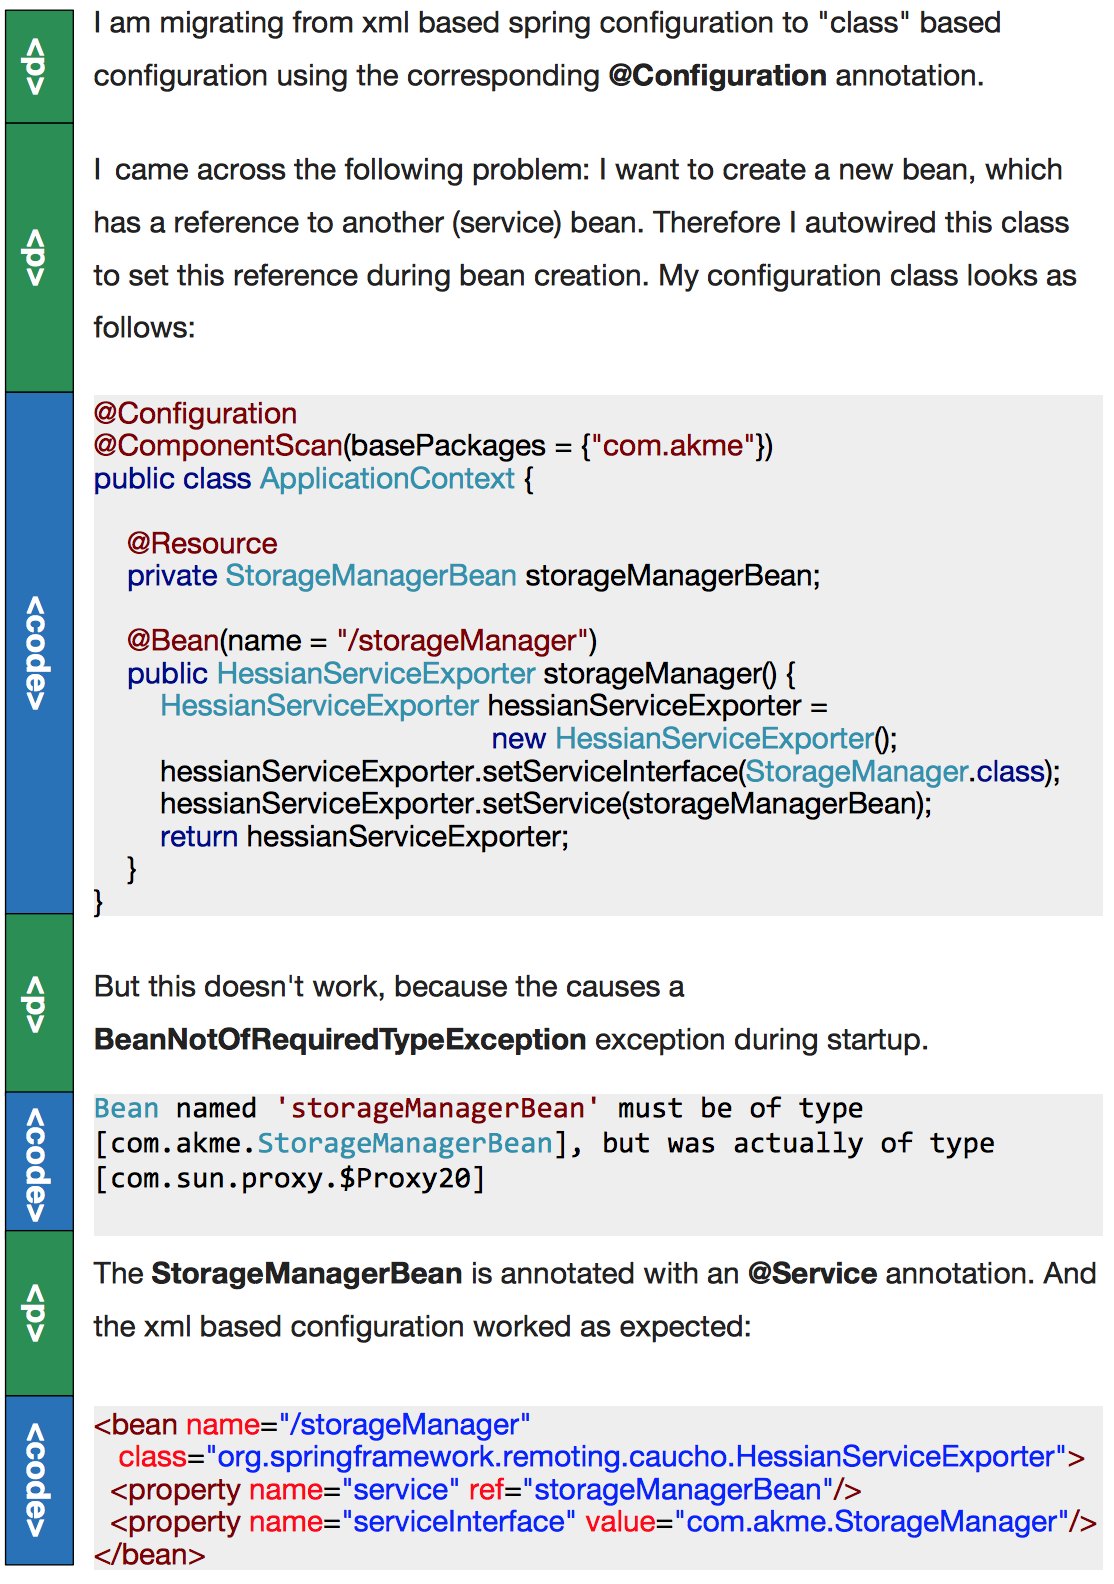
\includegraphics[width=\textwidth]{stackOverflow}
	\caption{Example of Stack Overflow question with HTML tagging}
	\label{stackOverflow}
	\end{figure}

	\begin{figure}[htbp]
	\centering
	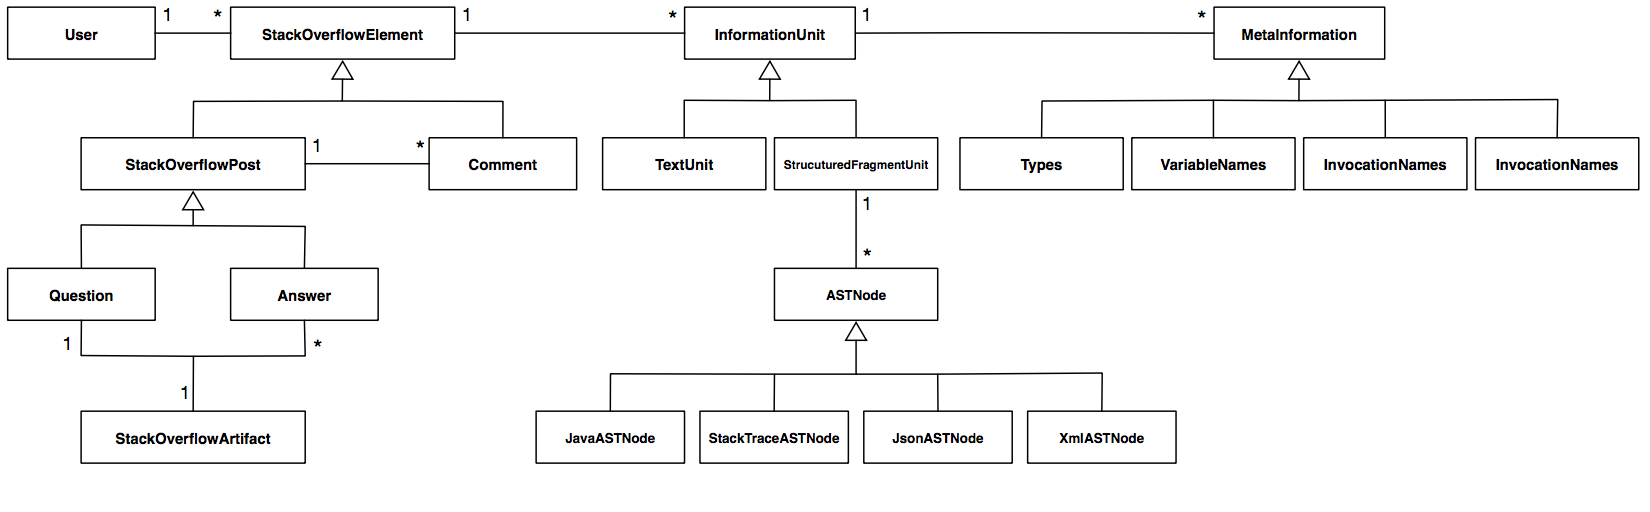
\includegraphics[width=\textwidth,height=5cm]{stormed}
	\caption{Stormed Object Model of the dataset}
	\label{stormed}
	\end{figure}

	Stormed provides us with a complete damp of Stack Overflow discussions, where each discussion is modeled as a heterogeneous abstract syntax, which allows us to distinguish between the textual part (natural language), and the code part. Moreover, Stormed parses the code part and identifies the Java code even if the code is incomplete.
	\newpage
	\section{Language Model}

	A \textbf{Probabilistic Language Model (LM)} is a probability distribution over sequences of words. Given such a sequence of length m, it assigns a probability $P(w_{1},\ldots ,w_{m})$ to the whole sequence\footnote{\url{https://en.wikipedia.org/wiki/Language_model}}.\\
	The language model goal is to compute the probability of a sentence or sequence of words.
	\[P(W) = P(w_{1},w_2,w_3,w_4,w_5\dots w_n)\]
	A LM can also compute the probability of an upcoming word.
	\[P(w_5|w_1,w_2,w_3,w_4)\]
	A LM applies Markov Chain Assumption to compute $P(W)$
	\[P(w_1w_2\dots w_n) \approx \prod_{i} P(w_i|w_{i-k} \dots w_{i-1})\]
	Each component in the product is approximated
	\[P(w_i |w_1w_2\dots w_{i-1}) \approx P(w_i |w{i-k} \dots w_{i-1})\]
	\textbf{Bigram model} provides the conditional probability of a word given the previous word.
	\[P(w_i |w_1w_2 \dots w_{i-1})\approx P(w_i |w_{i-1})\]
	The bigram model can be extended to trigrams, 4-grams, 5-grams, \dots , n-grams.\\
	$P(w_i |w_{i-1}$ is the maximum likelihood estimation in a bigram where 
	\[P(w_{i}|w_{{i-1}})=\frac{count(w_{{i-1}},w_{i})} {count(w_{{i-1}})}\]
	\textbf{Example}\\
	Lets consider the following text:\\
	Hi I am John\\
	Hi John I am David\\
	Hi I am looking for John

	\[P(I|HI)\ = \frac{2}{3} = 0.67\]
	The probabilities of the sentence ``I like Italian food'' estimated by a bigram model is:
	\[P(like|I) \times P(Italian|like) \times P(food|Italian)= 0.00042\]
	To avoid underflow and to make multiplication faster, we use log space.
	\[log( p_1 \times p_2 \times p_3 \times p_4 ) = log p_1 + log p_2 + log p_3 + log p_4\]



	\section{Training the Language Model}
	In our approach we use the 3-Gram model, we tried the 4-Gram and the 5-Gram but there was no significant difference. As we said before, we differentiate between natural language and code, therefore, we create a language model for each as we can see in \cref{trainingLm}.\\

	\begin{figure}[htbp]
	\centering
	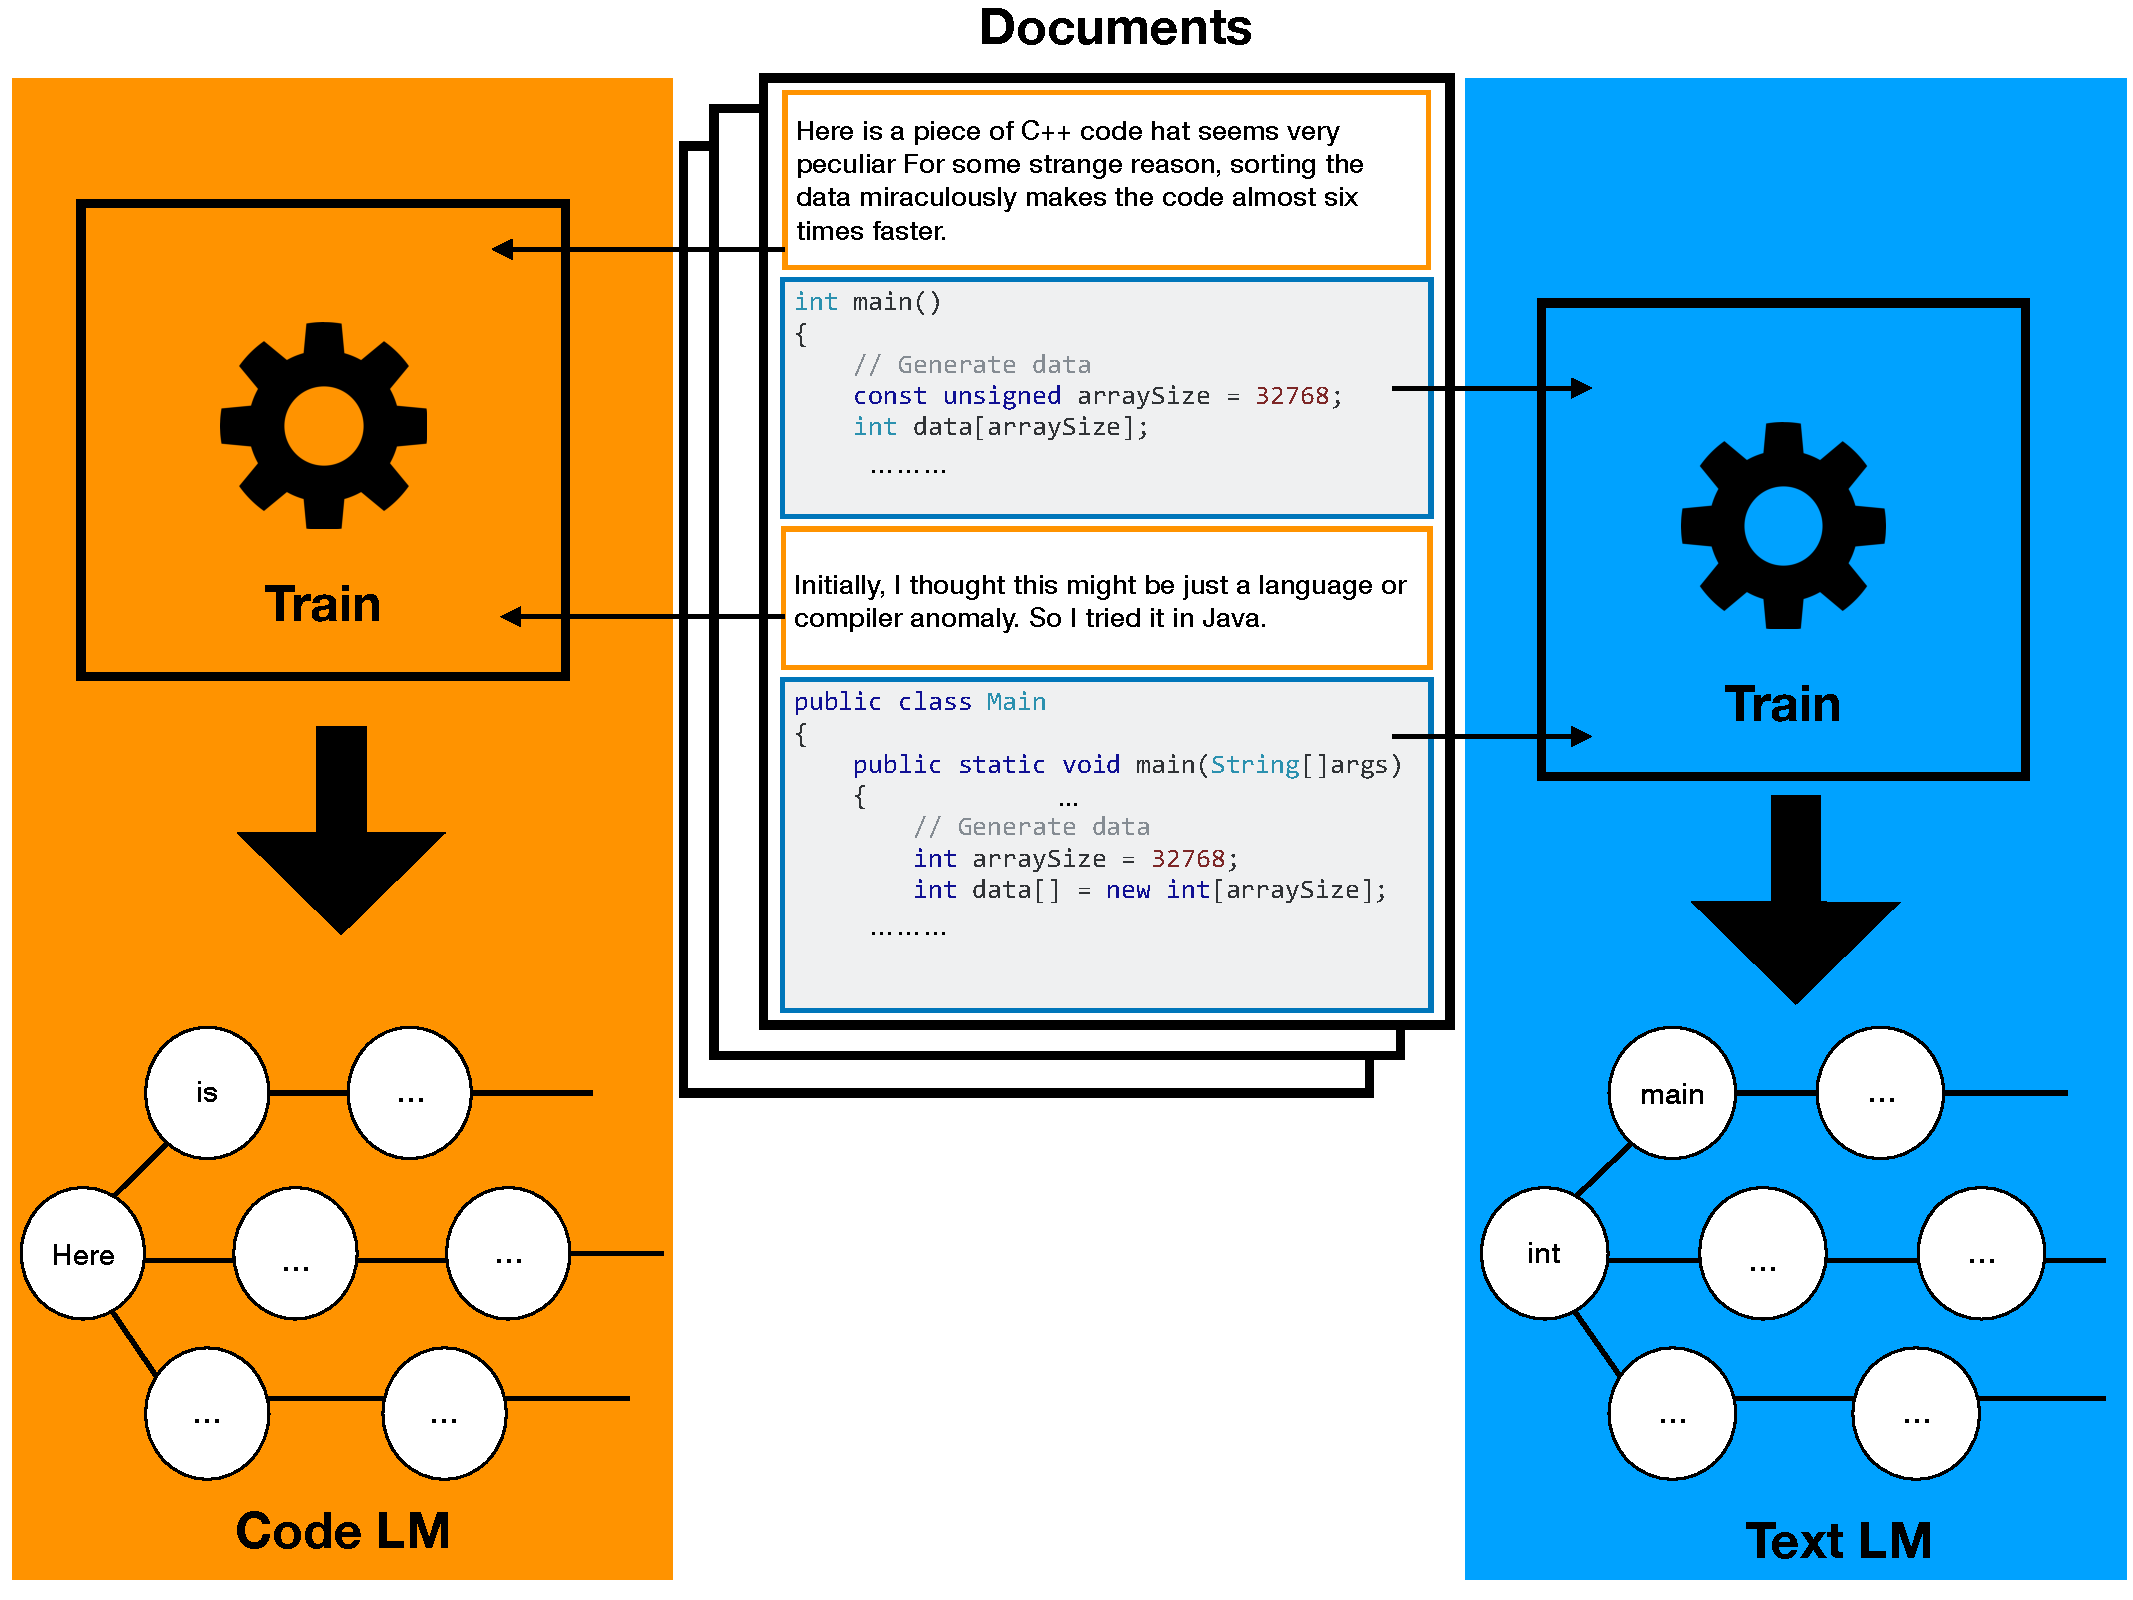
\includegraphics[width=\textwidth]{trainingLm}
	\caption{Training Language Model overview}
	\label{trainingLm}
	\end{figure}


	\begin{itemize}
		\item \textbf{Natural Language}: Once we have identify the textual part  of a document, we remove the stop words, since they are common words and they add noise to the LM, then we train the \emph{Natural Language LM} with the filtered text.
		\item \textbf{Code}: For the code part we use a similar process. We use ANTLR\footnote{\url{http://www.antlr.org}} parser to parse the code, then we remove all separators, since they add noise to the LM. \cref{FilterLM}\\
		The reason why we decide to remove the separators is because we had several situations, where a three curly brackets $\}\}\}$ or two curly brackets with any character $x\}\}$ were the most familiar 3-Gram. To avoid this noise we remove the separators from the code.
	\end{itemize}
	

	\begin{figure}[htbp]
	\centering
	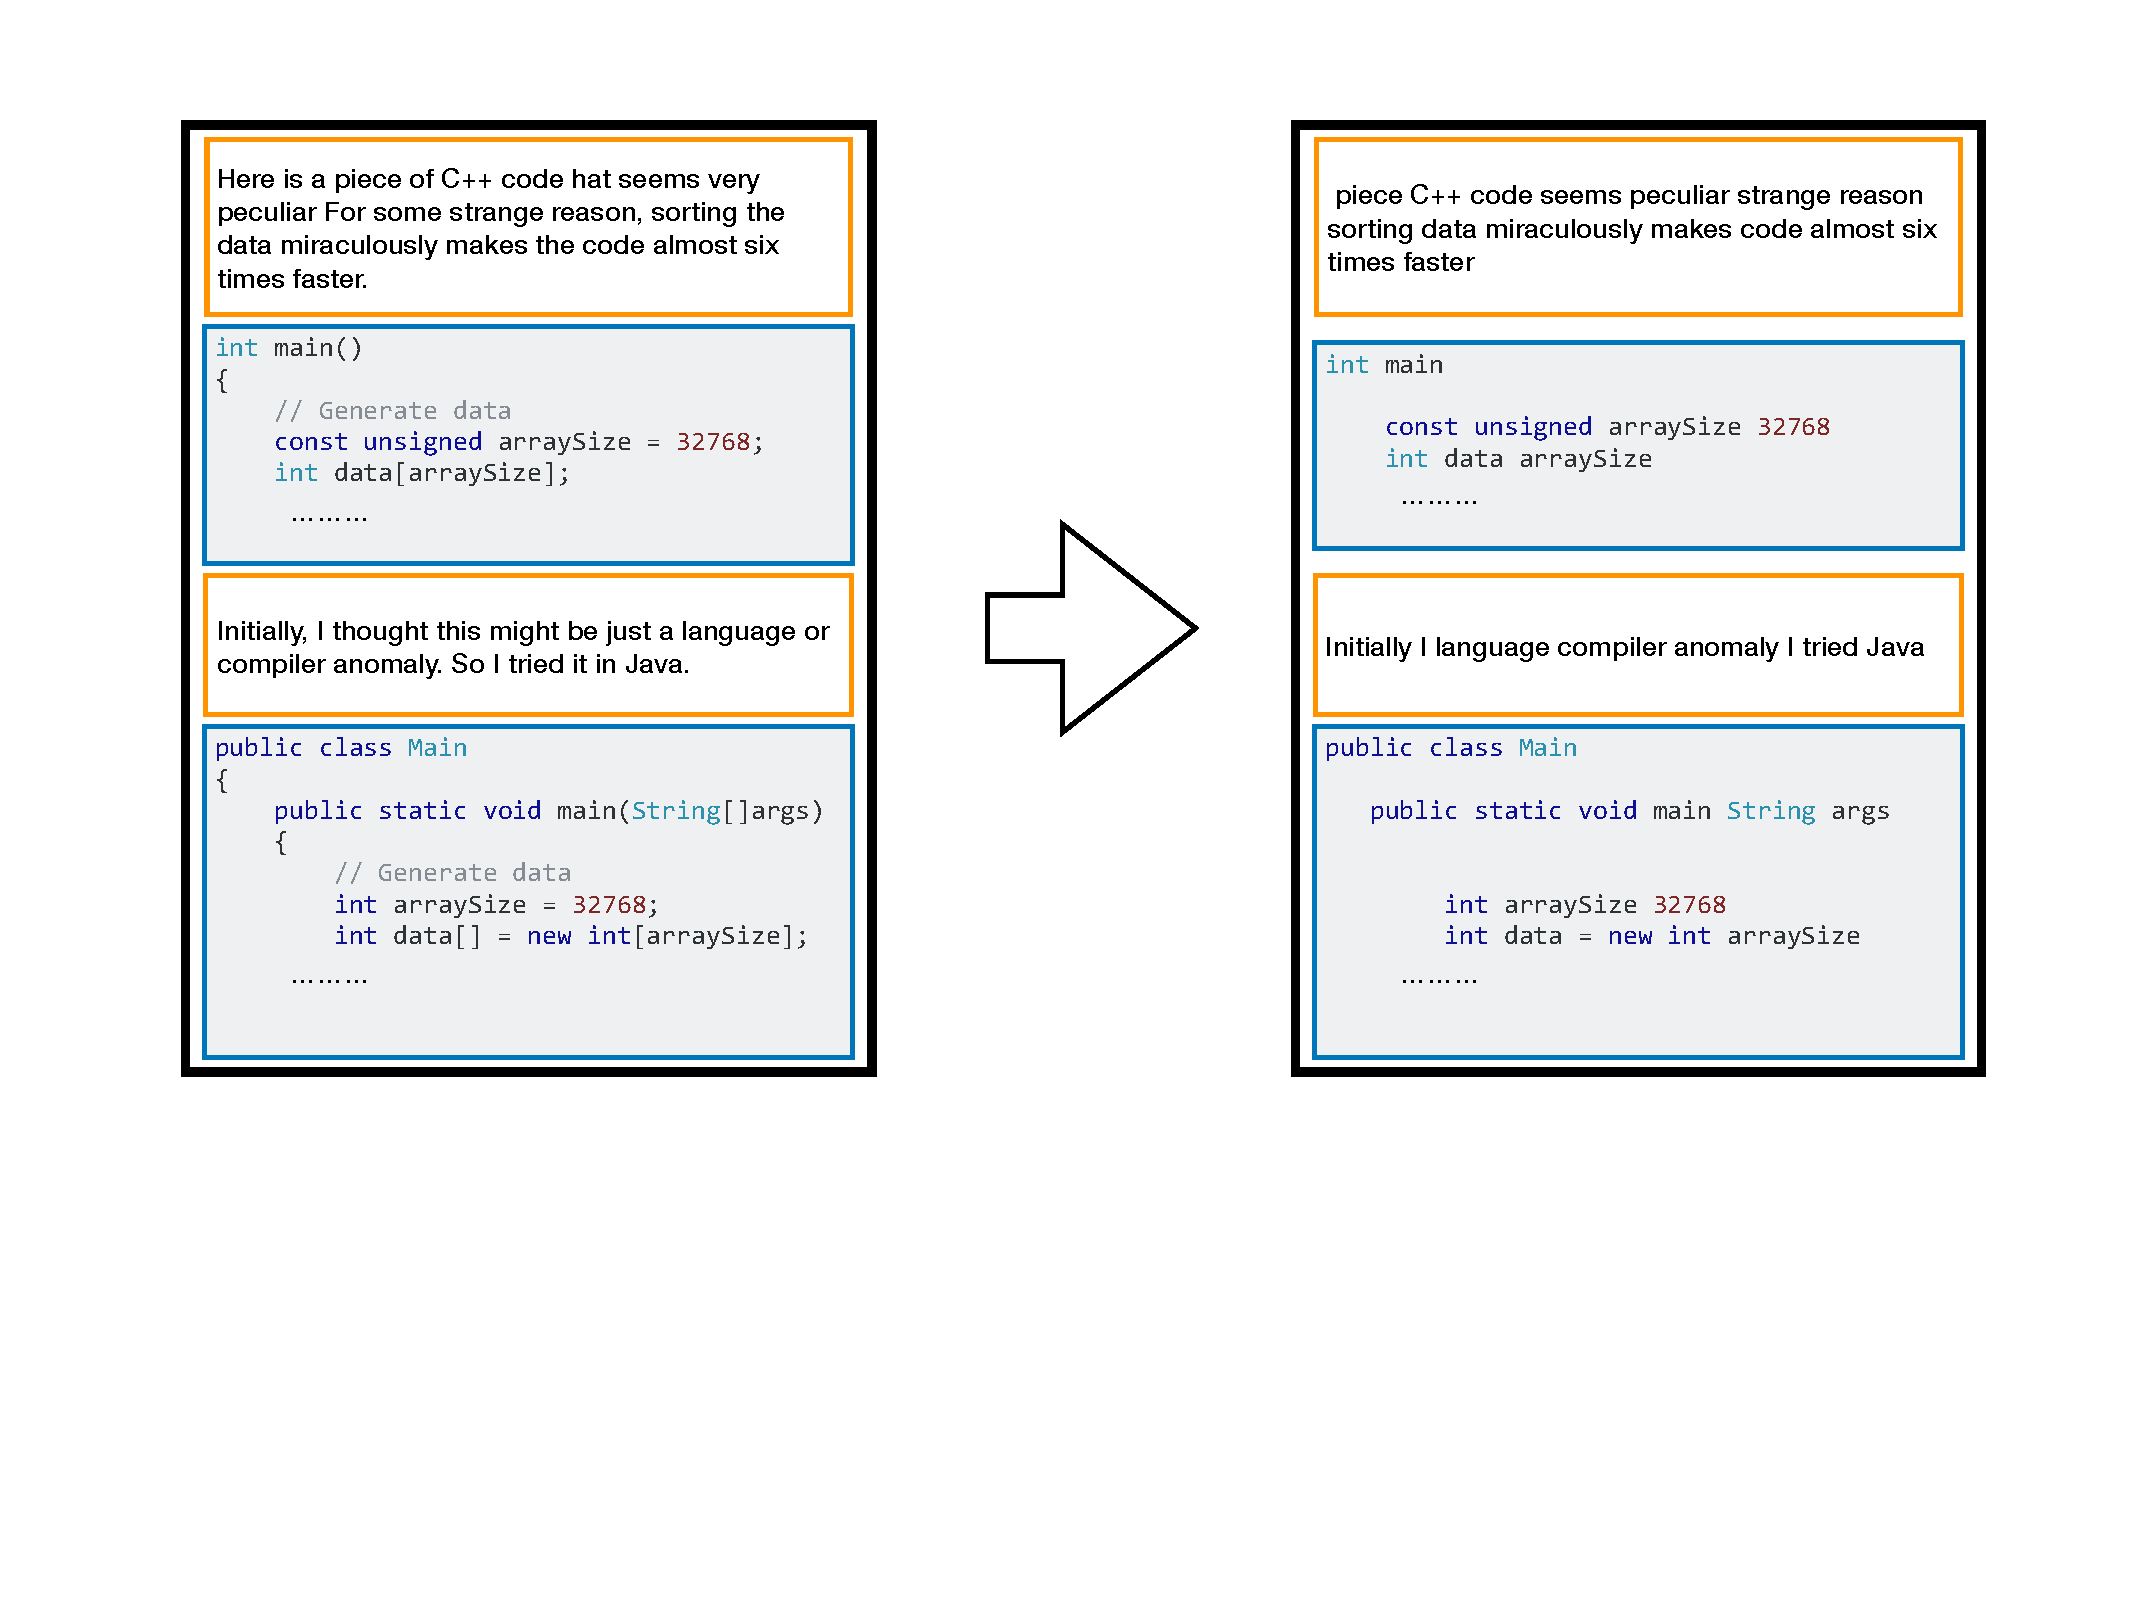
\includegraphics[width=\textwidth]{FilterLM}
	\caption{Filtering stop words and separators}
	\label{FilterLM}
	\end{figure}


	\section{Familiarity}
	We define the familiarity as the estimation of likelihood of a specified character sequence. But before estimating the familiarity, we need to do the following preprocessing steps:
	\begin{itemize}
		\item \textbf{Selecting \& Filtering}: As we did in the training phase, we use Stormed Island Parser\footnote{\url{https://stormed.inf.usi.ch}} \cite{Ponz2015a} to break down a document into text and code. We remove the stop words form the text, we parse the code\footnote{\url{http://www.antlr.org}} and we remove the separators, as shown in \cref{FilterLM}
		\item \textbf{3-Grams generating }: In \cref{3gram-generating} we can see that each chunk of code or text is transformed to a 3-Gram model, and then we calculate the familiarity of each N-Gram as shown in \cref{3gram-evaluating}.
			
			\begin{figure}[htbp]
			\centering
			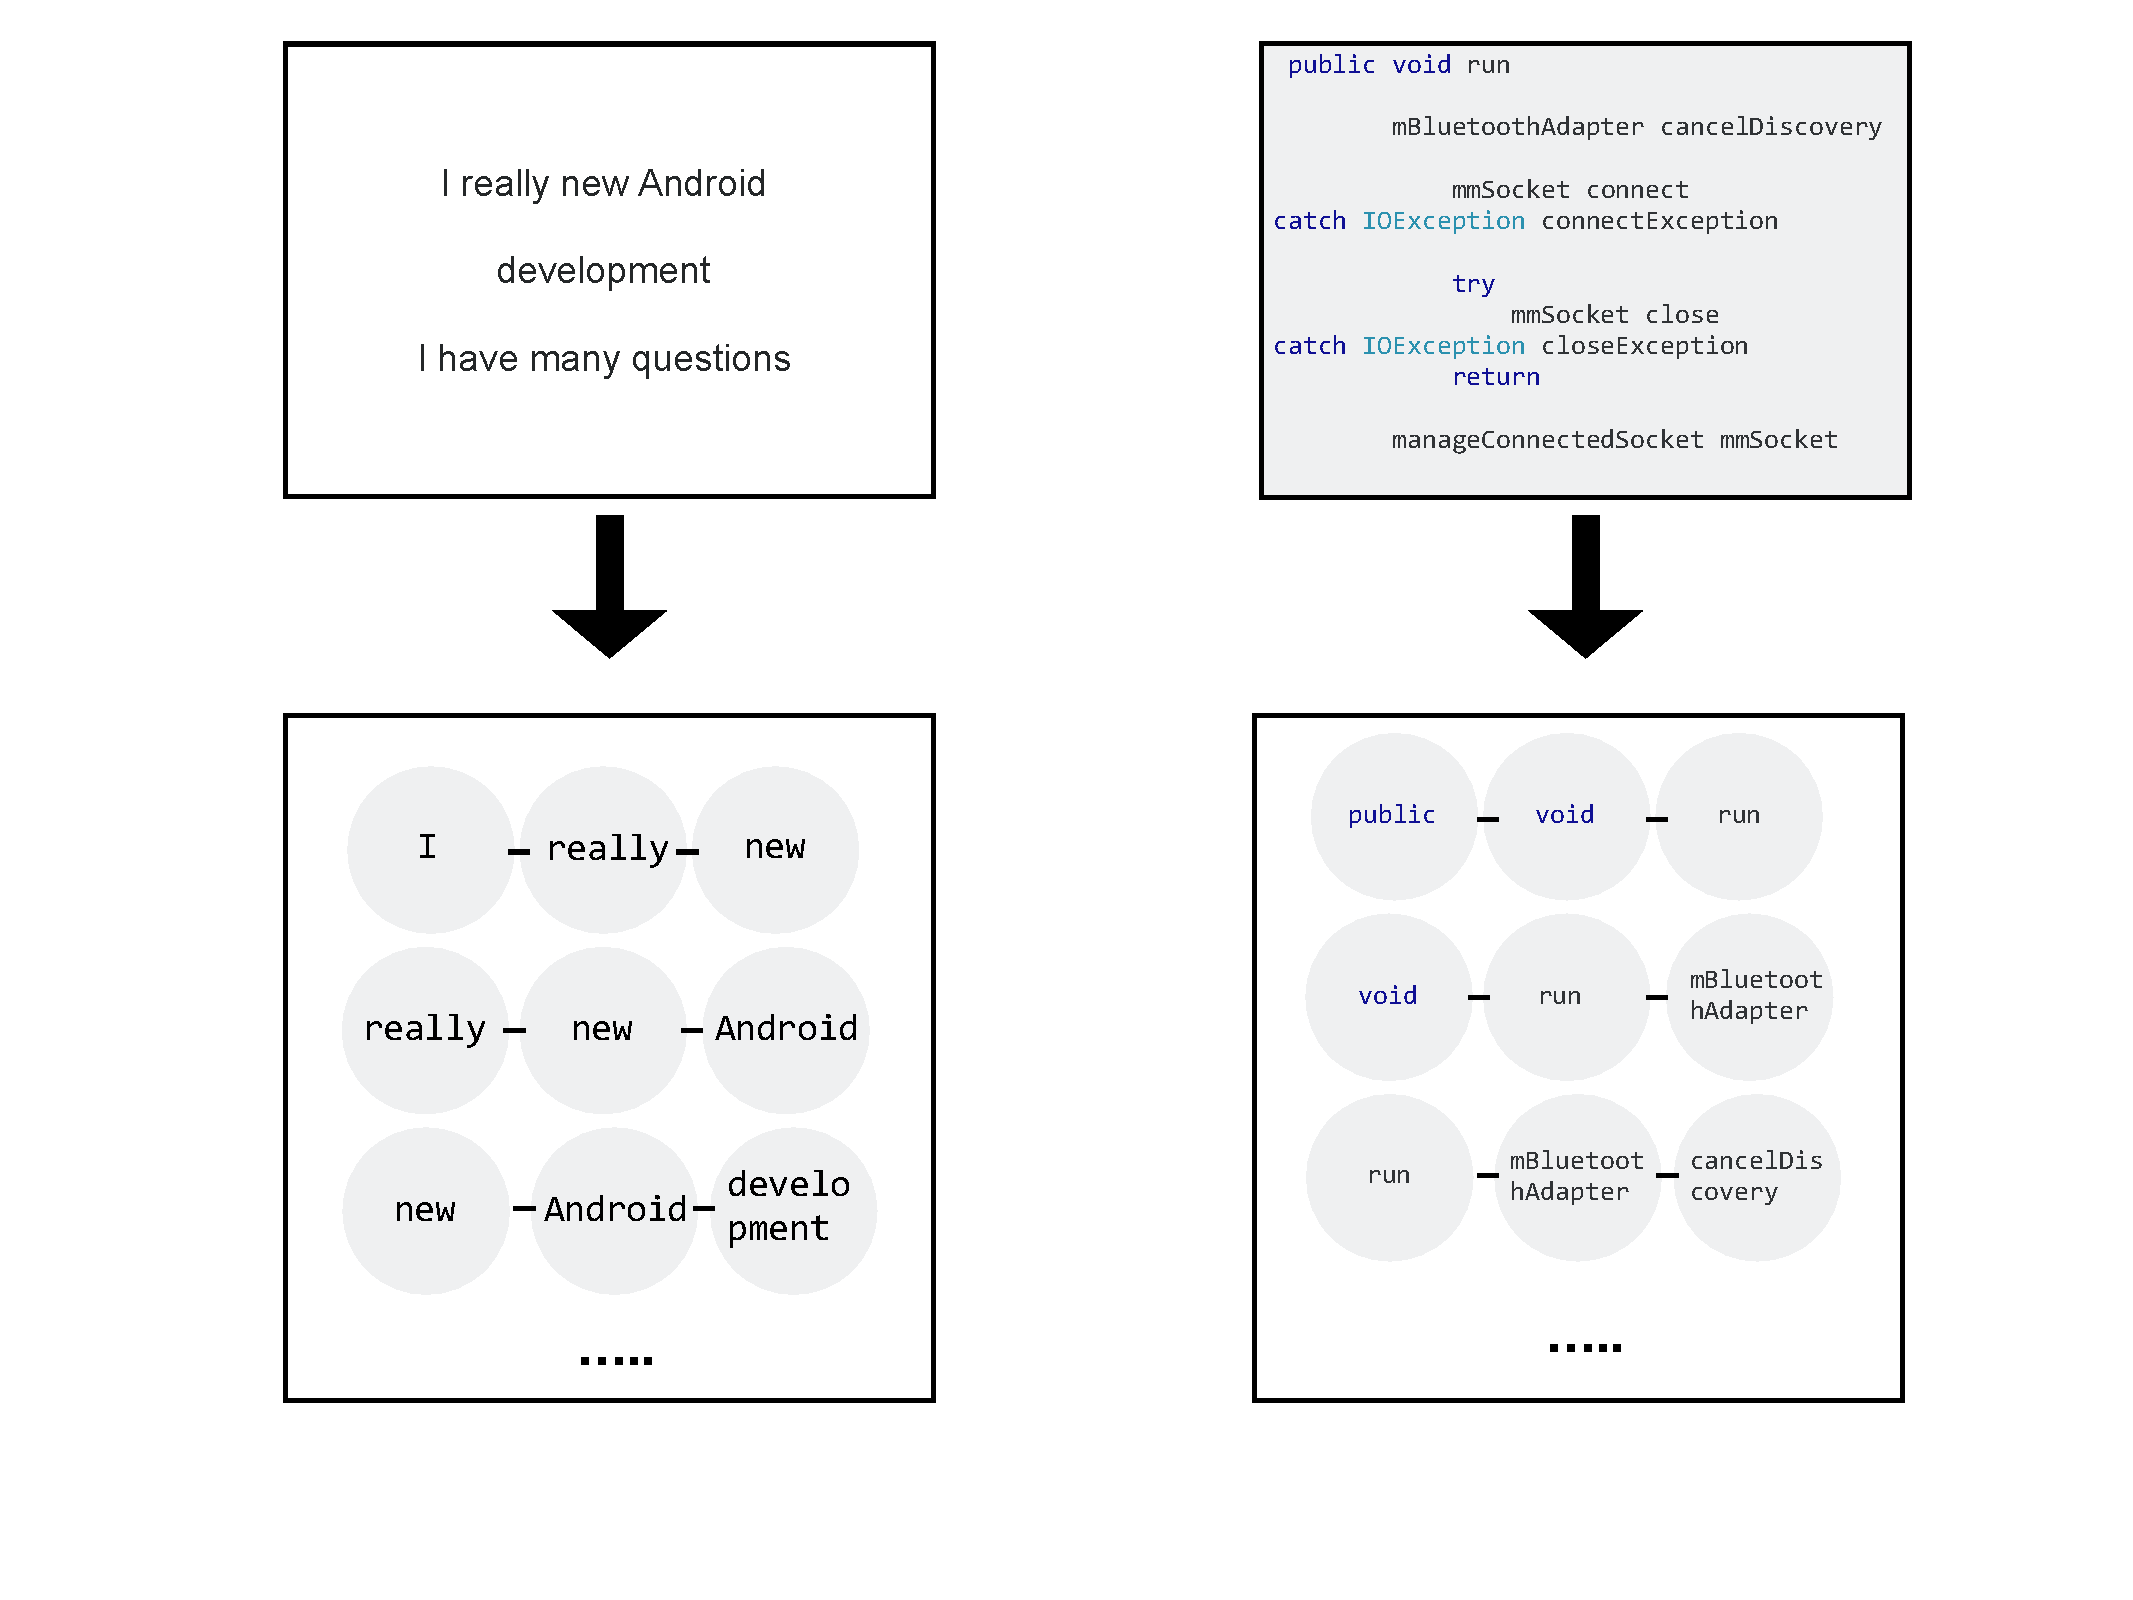
\includegraphics[width=\textwidth]{3gram-generating}
			\caption{3-Gram generating process}
			\label{3gram-generating}
			\end{figure}

			\begin{figure}[htbp]
			\centering
			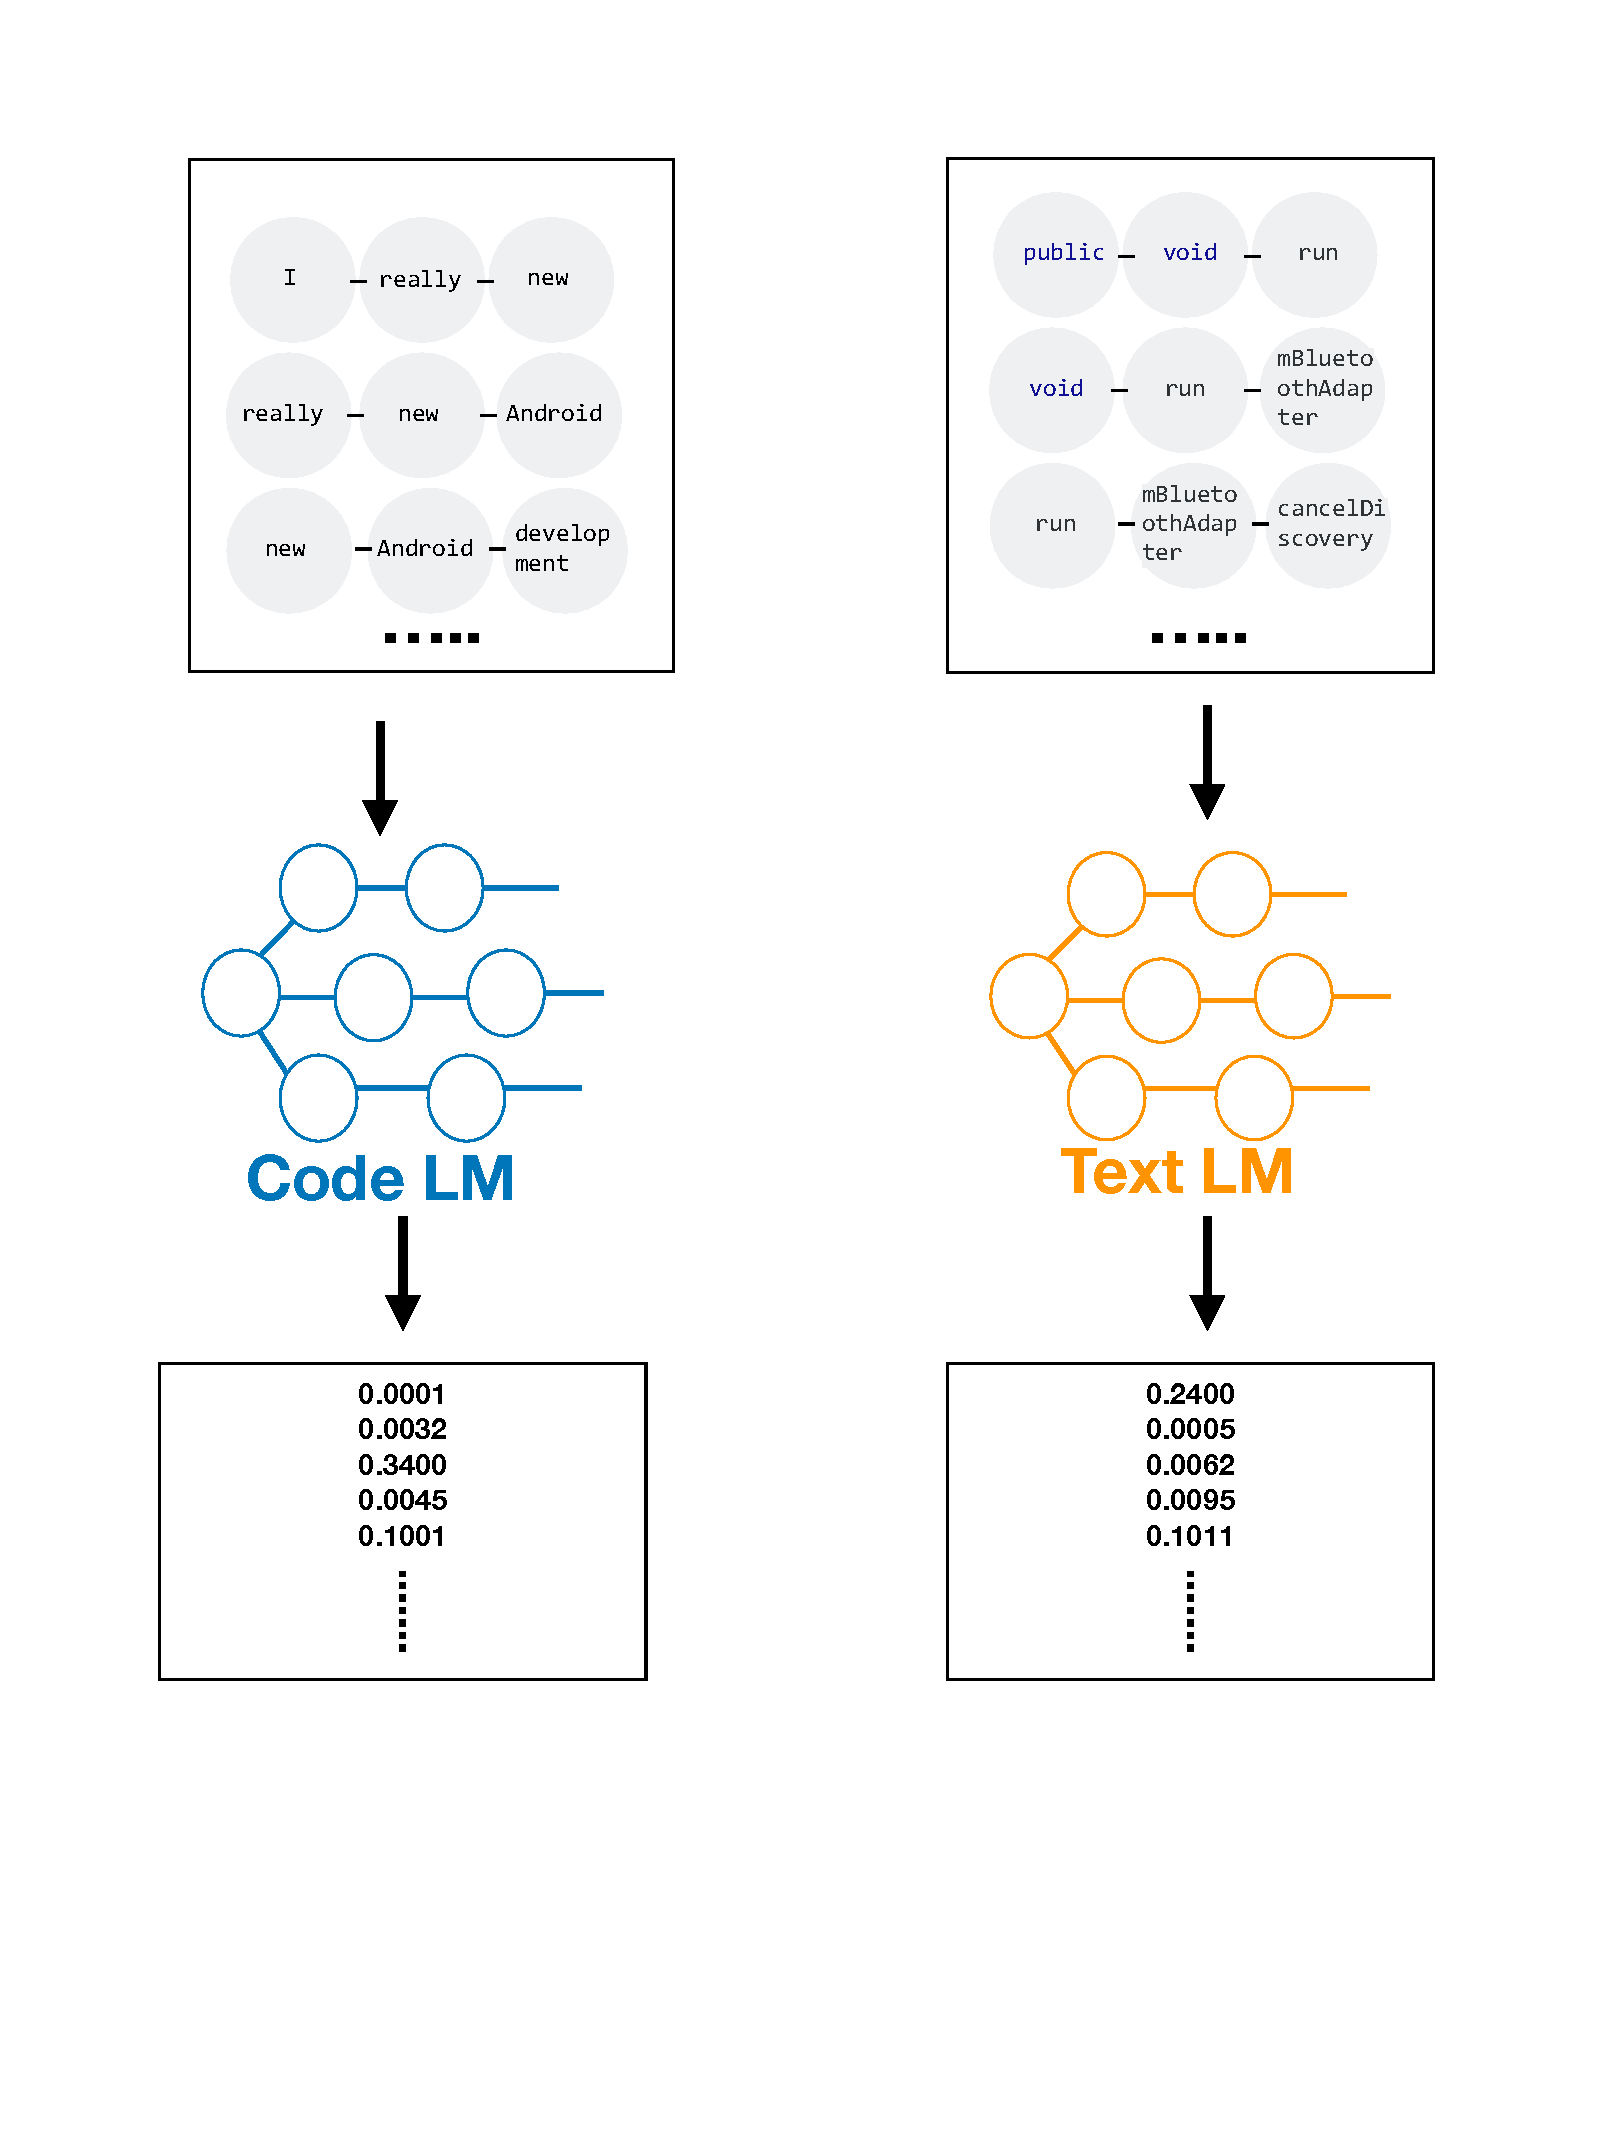
\includegraphics[width=\textwidth]{3gram-evaluating}
			\caption{3-Gram evaluating process}
			\label{3gram-evaluating}
			\end{figure}	
	
	
		\item \textbf{Familiarity aggregation}: Now that we have retrieved the familiarity of each 3-Gram of a given document, we need to aggregate them in one value. The trivial way is to multiply all the probabilities to get one value, but this approach is biased by the document length.\\
		As we can see in \cref{aggregation-by-multiplication} we have 2 documents, a and b, where \emph{document b} contains twice {document a}s' text. We expect to have the familiarity in both documents must be the same since they have the same text, even if in \emph{document b} the text is duplicated.\\ 
			\end{itemize}
		\begin{figure}[htbp]
			\centering
			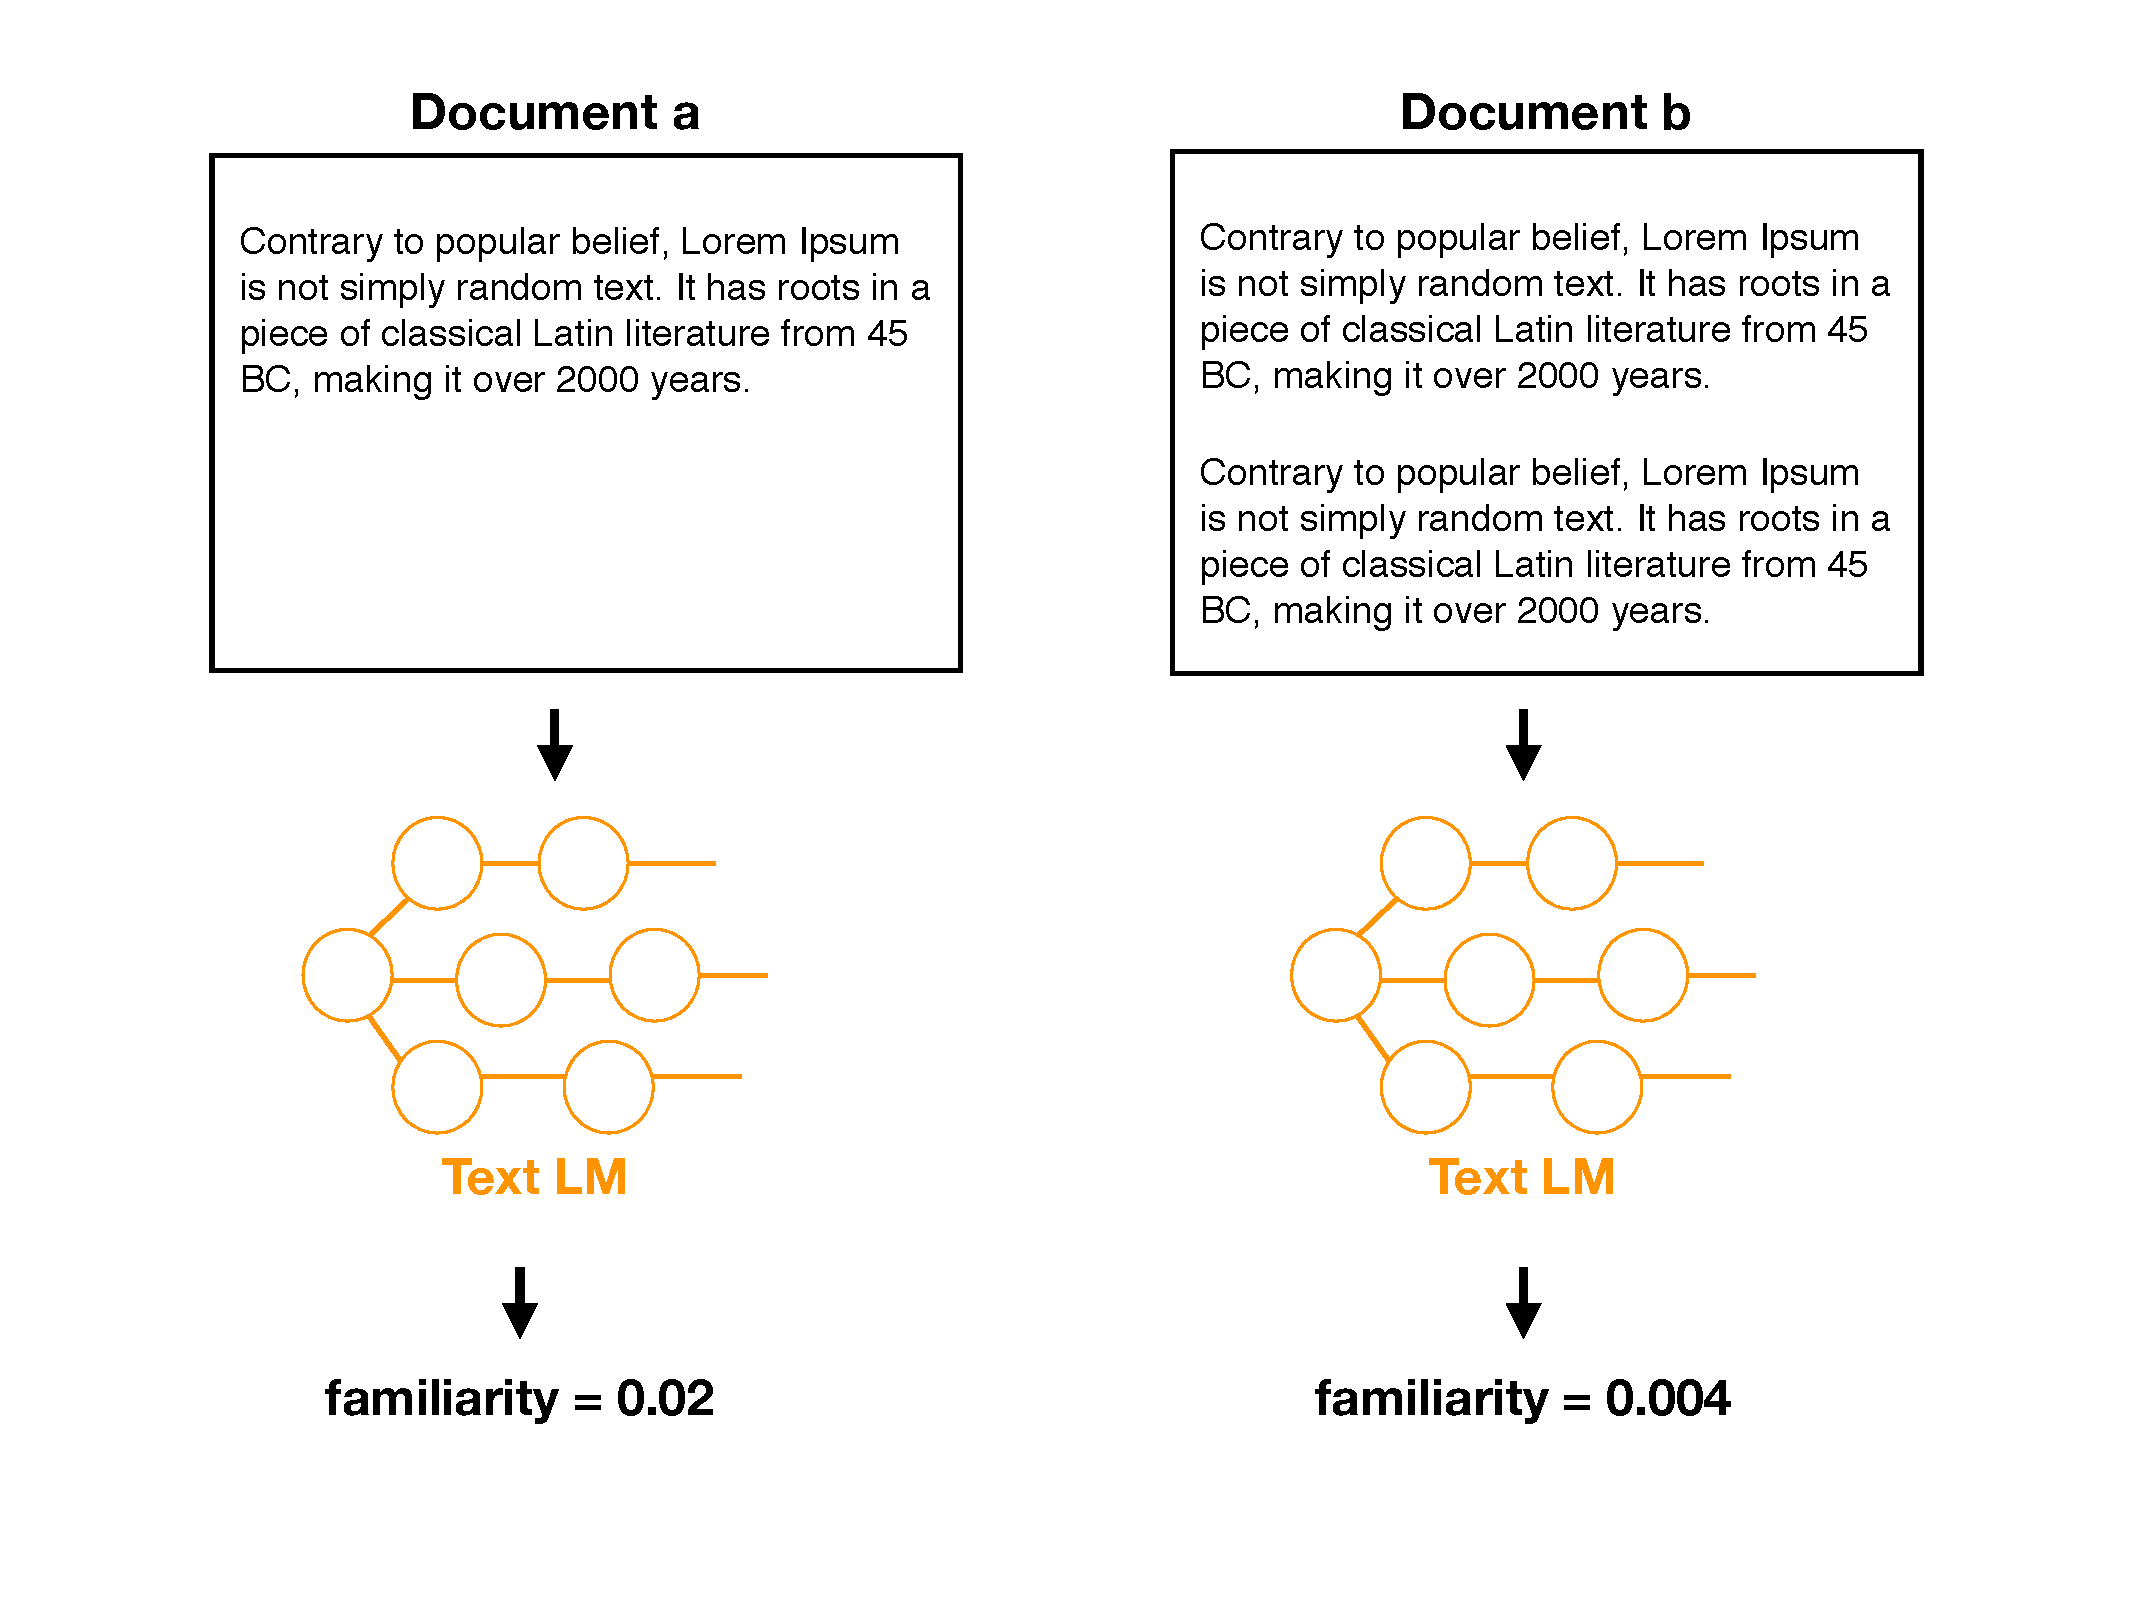
\includegraphics[width=\textwidth]{aggregation-by-multiplication}
			\caption{Aggregating probabilities by multiplication}
			\label{aggregation-by-multiplication}
			\end{figure}


			\begin{figure}[htbp]
			\centering
			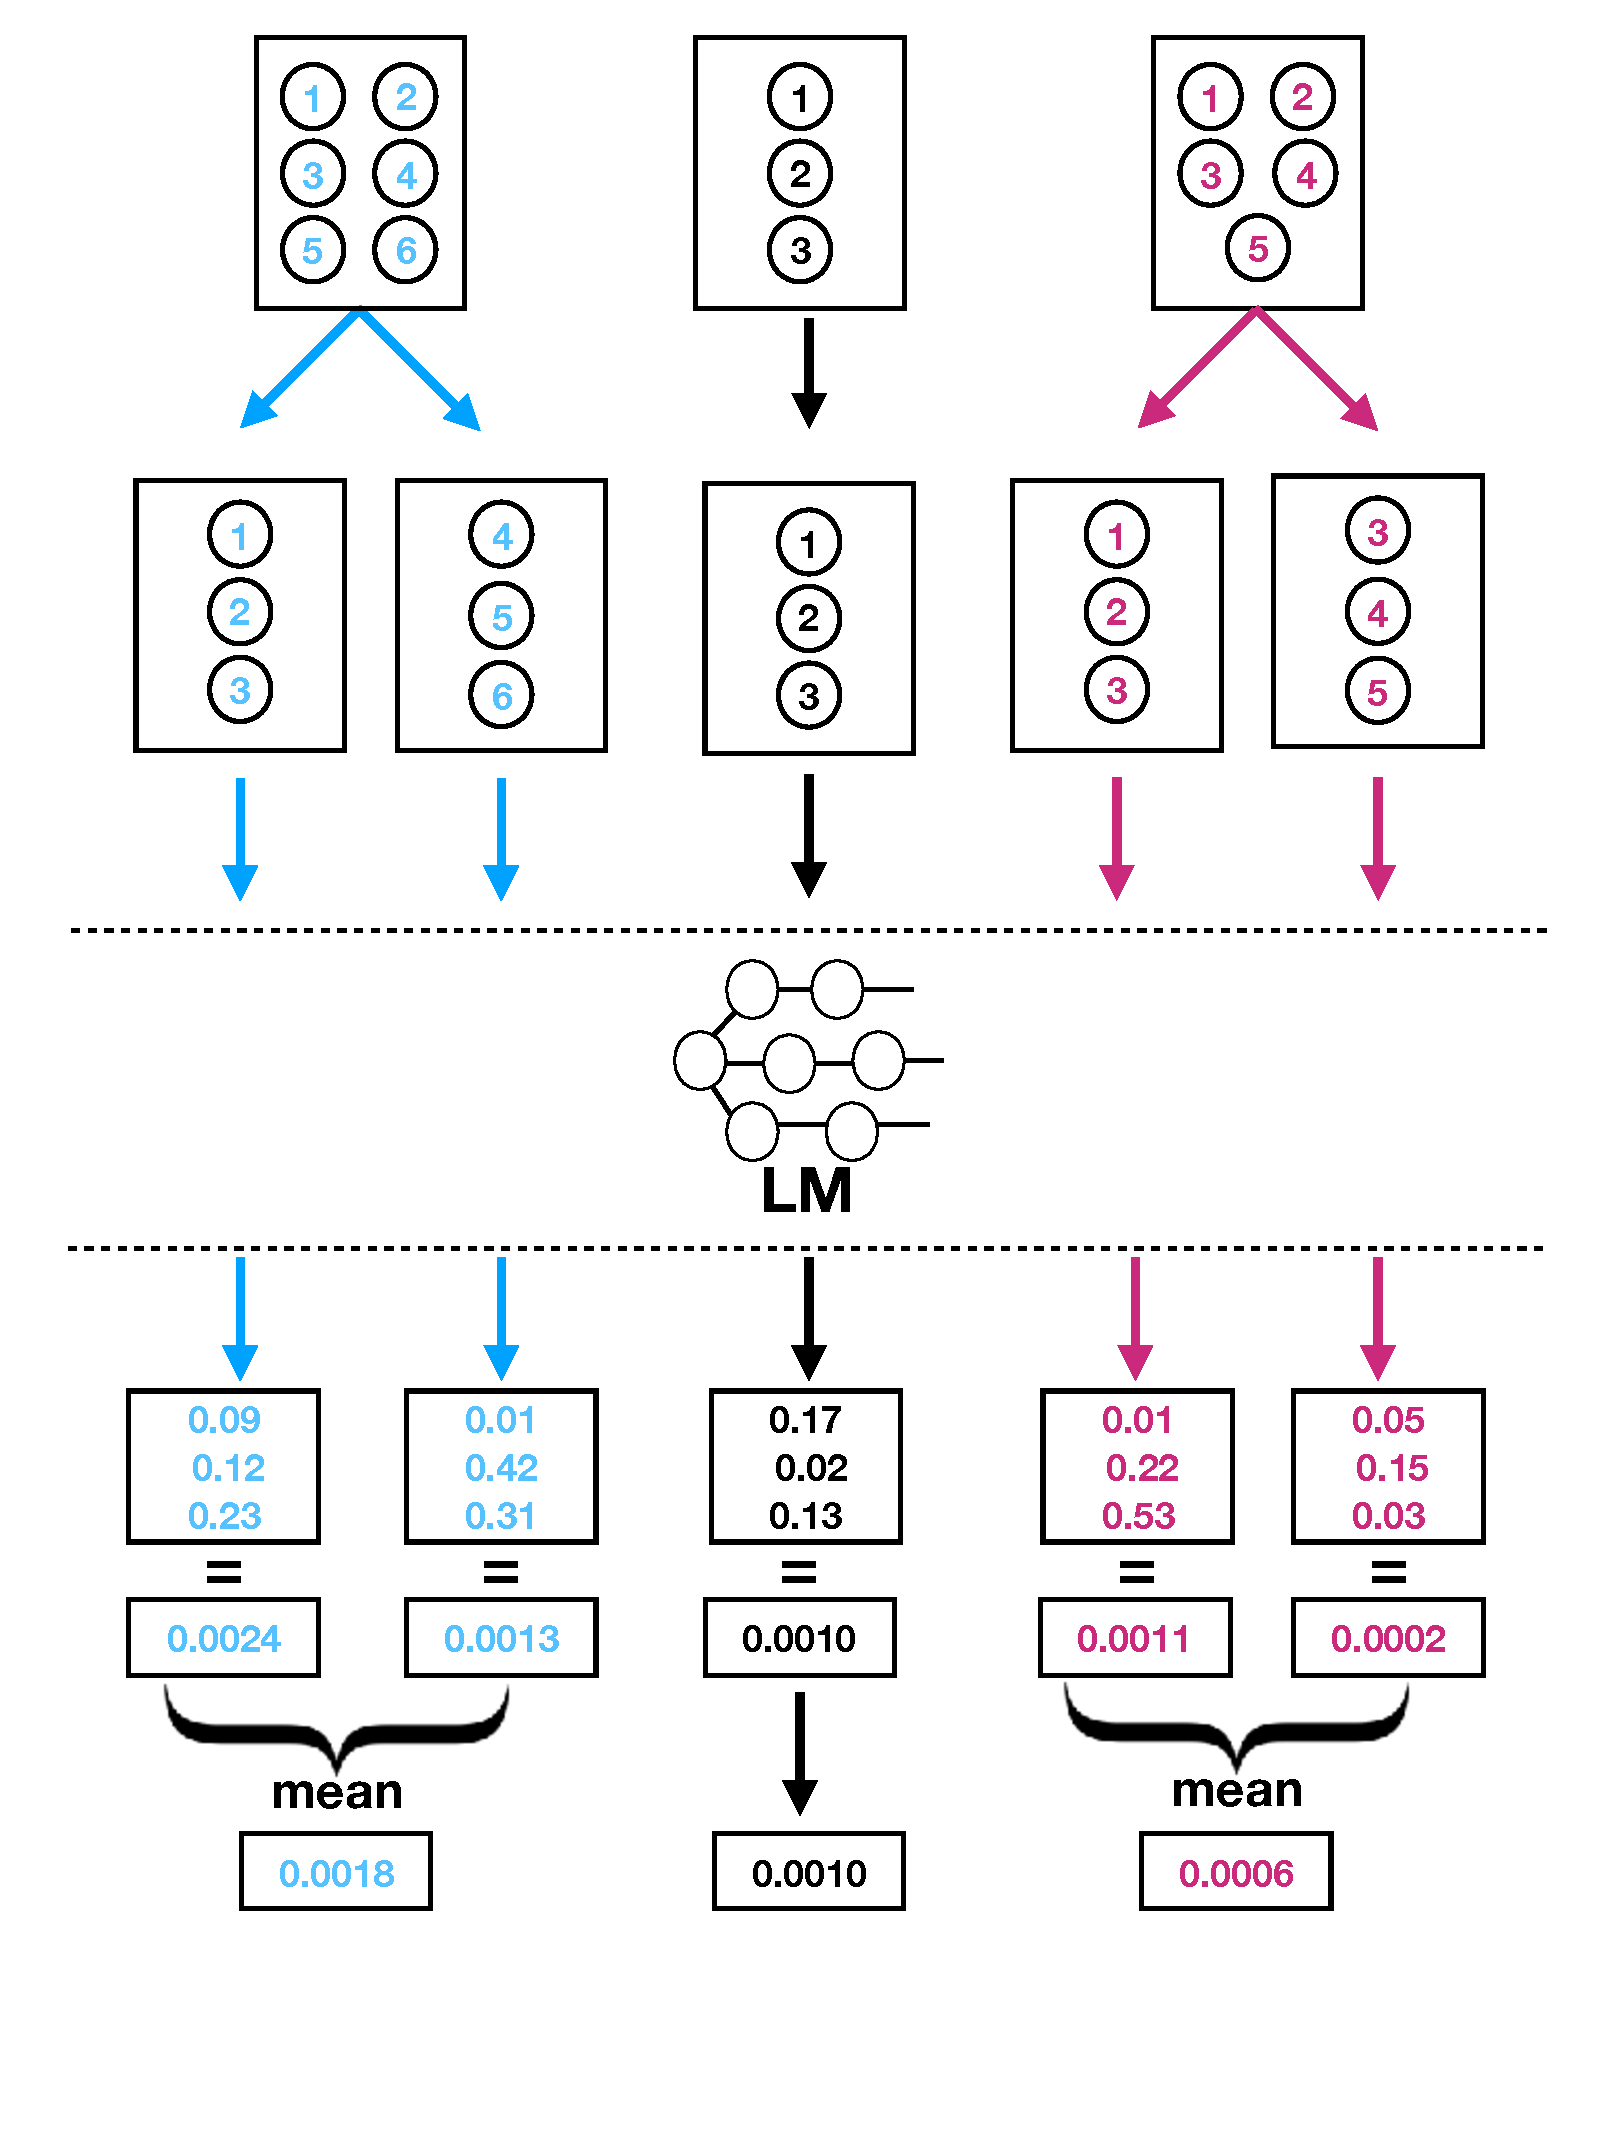
\includegraphics[width=\textwidth]{aggregation-by-mean}
			\caption{Aggregating probabilities by mean}
			\label{aggregation-by-mean}
			\end{figure}
		
		Given a set of documents with different length, the shortest documents turns out to be the most familiar. This approach is valid if all documents have the same length, which is not the case with the documents that we are dealing with, since they have heterogeneous length. 
		\newpage
		We tackle this problem by introducing a new approach to aggregate the probabilities \cref{aggregation-by-mean}.
		The approach consists 5 steps: 
		\begin{itemize}
			\item \textbf{step 1}: We select from the set the document with the smallest number of 3-Gram, say of length m.
			\item \textbf{step 2}: We split each document into chunks of length m.
			\item \textbf{step 3}: For each chunk we calculate the familiarity of its 3-Grams
			\item \textbf{step 4}: Now that all chunks have the same size, we calculate the familiarity of a chunk by multiplying the probability of all its 3-Grams
			\item \textbf{step 5}: Is the last step, where the familiarity of a document is derived from the mean of its chunks familiarity.
		\end{itemize}

\section{Readability} 
	The document readability has a big impact on the comprehension effort. Two text documents can contain approximately the same information, but one text can be easy to read and the other one can be difficult to read, and it is the same for code. The following peace of code can be written on one line :

	\lstset{language=algebra,linewidth=0.95\linewidth,breaklines=true,numbers=left,
	basicstyle=\ttfamily,numberstyle=\tiny,escapeinside={//*}{\^^M},
	mathescape=true}
	\begin{lstlisting}
{"name":"mkyong.com","messages":["msg 1","msg 2"],"age":100}

	\end{lstlisting}

	
	But most likely developers will find it easier to read the indented code:\\

	 	\begin{lstlisting}
{
	"name":"mkyong.com",
	"messages":["msg 1","msg 2"],
	"age":100
}
	\end{lstlisting}
 
	As mentioned so far we distinguish between \emph{code readability} and \emph{text readability}. Therefor, we use different tools to calculate the readability of each. 
\newpage
\subsection{Accounting for Text Readability}
	The text readability score is calculated by the \textbf{Flesch-Kincaid} \footnote{\url{https://en.wikipedia.org/wiki/Flesch–Kincaid_readability_tests}} formula:
	

	\[0.39\left({\frac  {{\mbox{total words}}}{{\mbox{total sentences}}}}\right)+11.8\left({\frac  {{\mbox{total syllables}}}{{\mbox{total words}}}}\right)-15.59\]
	A higher scores indicate that the document is easier to read and a lower number indicates that the document is more difficult to read.\\ 
	Flesch-Kincaid score is scaled in 0-100 rage, but for convenience we normalize it to 0-1 range.The score can be interpreted as shown in the table below.
	
	\begin {table}[H]
	\begin{center}
    \begin{tabular}{| l | l | p{7cm} | }
    \hline
    \textbf{Score} & \textbf{School Level} & \textbf{Notes} \\ \hline
    $100.0-90.0$ & 5th grade & Very easy to read. Easily understood by an average 11-year-old student.\\ \hline
    $90.0-80.0$ & 6th grade & Easy to read. Conversational English for consumers.\\ \hline
 	$80.0-70.0$ & 7th grade & Fairly easy to read. \\ \hline
	$70.0-60.0$ & 8th \& 9th grade & Plain English. Easily understood by 13- to 15-year-old students.\\ \hline
	$60.0-50.0$ & 10th to 12th grade &  Fairly difficult to read.\\ \hline
	$50.0-30.0$ & College & Difficult to read.\\ \hline
	$30.0-0.0$ & College Graduate & Very difficult to read. Best understood by university graduates\\\hline

    \end{tabular}
	\end{center}
	\caption{Flesch-Kincaid score grade} \label{tab:Flesch-Kincaid} 
	\end{table}

\subsection{Accounting for Code Readability}

	To calculate the code readability we use \citet{Buse:2010:LMC:1850489.1850615} code readability metric, and tool\footnote{\url{http://www.arrestedcomputing.com/readability}}.
	 Buse and Weimer determined a set of code features that are predictive of readability. The features are listed in the \cref{tab:Buse and Weimer}.

	\begin {table}[H]
	\begin{center}
    \begin{tabular}{ | l | }
    \hline
    \textbf{Feature Name}\\ \hline
	line length (\# characters)\\ \hline
 	\# identifiers\\ \hline
 	identifier length\\ \hline
	indentation (preceding whitespace)\\ \hline
	\#keywords\\ \hline
	 \#numbers\\ \hline
	\#comments\\ \hline
	\#periods\\ \hline
	\#commas\\ \hline
	\#spaces\\ \hline
	\#parenthesis\\ \hline
	 \#arithmetic operators\\ \hline
	 \#comparison operators\\ \hline
	 \#assignments (=)\\ \hline
	 \#branches (if)\\ \hline
	 \#loops (for, while)\\ \hline
	 \#blank lines\\ \hline
	 \#occurrences of any single character\\ \hline
	 \#occurrences of any single identifier\\ \hline
    \end{tabular}
	\end{center}
		\caption{Buse and Weimer code features \\ (Read “\#” as “number of ...”)} \label{tab:Buse and Weimer} 
	\end{table}

	Buse and Weimer's readability score is scaled in 0-1 range, where a higher scores indicate that the code is easier to read and a lower number indicates that the code is more difficult to read.


\section{Accounting Comprehension Effort }

\[\frac{(r_{c}\times f_{c}) + (r_{t} \times f_{t})}{2} \]
	
\chapter{Study Design}
	\section{Research Questions}
	\section{Data Collection and Analysis}	
	\section{Replication Package}

\chapter{Results}

\chapter{Threats to Validity}

\chapter{Conclusion}

\chapter[Short title]{A chapter title which will run over two lines --- it's for
  testing purpose}


\textbf{Theorem 1 (Residue Theorem).}
Let $f$ be analytic in the region $G$ except for the isolated singularities $a_1,a_2,\ldots,a_m$. If $\gamma$ is a closed rectifiable curve in $G$ which does not pass through any of the points $a_k$ and if $\gamma\approx 0$ in $G$ then
\[
\frac{1}{2\pi i}\int_\gamma f = \sum_{k=1}^m n(\gamma;a_k) \text{Res}(f;a_k).
\]
\textbf{Theorem 2 (Maximum Modulus).}
\emph{Let $G$ be a bounded open set in $\mathbb{C}$ and suppose that $f$ is a continuous function on $G^-$ which is analytic in $G$. Then}
\[
\max\{|f(z)|:z\in G^-\}=\max \{|f(z)|:z\in \partial G \}.
\]

\section[third]{A very very long section, titled ``The third section'', with
  a rather  short text alternative (third)}



\nocite{*}

\appendix %optional, use only if you have an appendix



\backmatter

\chapter{Glossary} %optional

%\bibliographystyle{alpha}
%\bibliographystyle{dcu}
\bibliographystyle{plainnat}
\bibliography{biblio}

%\cleardoublepage
%\theindex %optional, use only if you have an index, must use
	  %\makeindex in the preamble


\end{document}
